\documentclass{tufte-handout}

\usepackage{amsmath}
\usepackage{graphicx}
\setkeys{Gin}{width=\linewidth,totalheight=\textheight,keepaspectratio}

\usepackage{booktabs}
\usepackage{units}
\usepackage{fancyvrb}
\fvset{fontsize=\normalsize}
\usepackage{multicol}
\usepackage{lipsum}
\PassOptionsToPackage{dvipsnames}{xcolor}
\usepackage{xcolor}
\usepackage{amsmath, amsthm, thmtools}
\usepackage{amssymb}
\usepackage{cleveref}
\usepackage{csquotes}
\geometry{
  marginparwidth=60mm % width of margin notes
}
%%%%%%%%% mathematical bold  %%%%%%%%%%%%%%%%%

\newcommand{\bA}{\mathbb{A}}
\newcommand{\bB}{\mathbb{B}}
\newcommand{\bC}{\mathbb{C}}
\newcommand{\Cs}{\bC^\times}
\newcommand{\bD}{\mathbb{D}}
\newcommand{\bE}{\mathbb{E}}
\newcommand{\F}{\mathbb{F}}
\newcommand{\bF}{\mathbb{F}}
\newcommand{\bG}{\mathbb{G}}
\newcommand{\bH}{\mathbb{H}}
\newcommand{\bI}{\mathbb{I}}
\newcommand{\bJ}{\mathbb{J}}
\newcommand{\bK}{\mathbb{K}}
\newcommand{\bL}{\mathbb{L}}
\newcommand{\bM}{\mathbb{M}}
\newcommand{\N}{\mathbb{N}}
\newcommand{\bO}{\mathbb{O}}
\newcommand{\bP}{\mathbb{P}}
\newcommand{\bp}{\mathbb{p}}
\newcommand{\Q}{\mathbb{Q}}
\newcommand{\R}{\mathbb{R}}
\newcommand{\bS}{\mathbb{S}}
\newcommand{\bT}{\mathbb{T}}
\newcommand{\bU}{\mathbb{U}}
\newcommand{\bV}{\mathbb{V}}
\newcommand{\bW}{\mathbb{W}}
\newcommand{\bX}{\mathbb{X}}
\newcommand{\bY}{\mathbb{Y}}
\newcommand{\Z}{\mathbb{Z}}

%%%%%%%%% calligraphic %%%%%%%%%%%%%%%%%%%%%%%

\newcommand{\mc}[1]{\mathcal{#1}}
\newcommand{\cA}{\mathcal{A}}
\newcommand{\cB}{\mathcal{B}}
\newcommand{\cC}{\mathcal{C}}
\newcommand{\cD}{\mathcal{D}}
\newcommand{\cE}{\mathcal{E}}
\newcommand{\cF}{\mathcal{F}}
\newcommand{\cG}{\mathcal{G}}
\newcommand{\cH}{\mathcal{H}}
\newcommand{\cI}{\mathcal{I}}
\newcommand{\cJ}{\mathcal{J}}
\newcommand{\cK}{\mathcal{K}}
\newcommand{\cL}{\mathcal{L}}
\newcommand{\cM}{\mathcal{M}}
\newcommand{\cm}{\mathcal{m}}
\newcommand{\cN}{\mathcal{N}}
\newcommand{\cO}{\mathcal{O}}
\newcommand{\cP}{\mathcal{P}}
\newcommand{\cQ}{\mathcal{Q}}
\newcommand{\cR}{\mathcal{R}}
\newcommand{\cS}{\mathcal{S}}
\newcommand{\cT}{\mathcal{T}}
\newcommand{\cU}{\mathcal{U}}
\newcommand{\cV}{\mathcal{V}}
\newcommand{\cW}{\mathcal{W}}
\newcommand{\cX}{\mathcal{X}}
\newcommand{\cY}{\mathcal{Y}}
\newcommand{\cZ}{\mathcal{Z}}

%%%%%%%%% mathematical fraktur  %%%%%%%%%%%%%%

\newcommand{\mf}[1]{\mathfrak{#1}}
\newcommand{\fa}{\mathfrak{a}}
\newcommand{\fb}{\mathfrak{b}}
\newcommand{\fc}{\mathfrak{c}}
\newcommand{\fA}{\mathfrak{A}}
\newcommand{\fB}{\mathfrak{B}}
\newcommand{\fC}{\mathfrak{C}}
\newcommand{\fD}{\mathfrak{D}}
\newcommand{\fE}{\mathfrak{E}}
\newcommand{\fF}{\mathfrak{F}}
\newcommand{\fG}{\mathfrak{G}}
\newcommand{\fH}{\mathfrak{H}}
\newcommand{\fI}{\mathfrak{I}}
\newcommand{\fJ}{\mathfrak{J}}
\newcommand{\fK}{\mathfrak{K}}
\newcommand{\fL}{\mathfrak{L}}
\newcommand{\fm}{\mathfrak{m}}
\newcommand{\fN}{\mathfrak{N}}
\newcommand{\fO}{\mathfrak{O}}
\newcommand{\fp}{\mathfrak{p}}
\newcommand{\fQ}{\mathfrak{Q}}
\newcommand{\fq}{\mathfrak{q}}
\newcommand{\fR}{\mathfrak{R}}
\newcommand{\fS}{\mathfrak{S}}
\newcommand{\fT}{\mathfrak{T}}
\newcommand{\fU}{\mathfrak{U}}
\newcommand{\fV}{\mathfrak{V}}
\newcommand{\fW}{\mathfrak{W}}
\newcommand{\fX}{\mathfrak{X}}
\newcommand{\fY}{\mathfrak{Y}}
\newcommand{\fZ}{\mathfrak{Z}}

%%%%%%%%%    math operators    %%%%%%%%%%%%%%%

\newcommand{\RP}{\mathbb{RP}^2}
\newcommand{\gen}[1]{\langle #1\rangle}
\newcommand{\Id}{\mathrm{Id}}
\DeclareMathOperator{\im}{im}
\DeclareMathOperator{\ggt}{ggT}
\DeclareMathOperator{\kgv}{kgV}
\DeclareMathOperator{\Aut}{Aut}
\DeclareMathOperator{\Hom}{Hom}
\DeclareMathOperator{\Iso}{Iso}
\DeclareMathOperator{\ord}{ord}
\DeclareMathOperator{\rad}{rad}
\DeclareMathOperator{\GL}{GL}
\DeclareMathOperator{\SL}{SL}
\DeclareMathOperator{\UT}{UT_3(\R)}
\DeclareMathOperator{\id}{id}
\DeclareMathOperator{\sgn}{sgn}
\DeclareMathOperator{\modn}{mod}
\DeclareMathOperator{\stab}{Stab_G}
\DeclareMathOperator{\Th}{Th}
\DeclareMathOperator{\On}{On}
\DeclareMathOperator{\Spec}{Spec}
\DeclareMathOperator{\coker}{coker}

%%%%%%%%%    further commands  %%%%%%%%%%%%%%%

\DeclareMathOperator{\nil}{nil}
\DeclareMathOperator{\Jac}{Jac}
\setlength{\headheight}{13.59999pt}

%%%%%%%%%    thmtools environments  %%%%%%%%%%%%%%%

\declaretheoremstyle[
shaded={
    rulecolor=Lavender!35,
    rulewidth=2pt,
    bgcolor=Lavender!25},
spaceabove=6pt, spacebelow=6pt,
headfont=\normalfont\bfseries, headindent=\parindent,
notefont=\mdseries, notebraces={(}{)},
bodyfont=\normalfont,
postheadspace=0.5em]{lav}

\declaretheoremstyle[
shaded={
    rulecolor=RoyalBlue!12,
    rulewidth=2pt,
    bgcolor=RoyalBlue!8},
spaceabove=6pt, spacebelow=6pt,
headfont=\normalfont\bfseries, headindent=\parindent,
notefont=\mdseries, notebraces={(}{)},
bodyfont=\normalfont,
postheadspace=0.5em]{blue}

\declaretheoremstyle[
shaded={
    rulecolor=RoyalBlue!8,
    rulewidth=2pt,
    bgcolor=RoyalBlue!5},
spaceabove=6pt, spacebelow=6pt,
headfont=\normalfont\bfseries, headindent=\parindent,
notefont=\mdseries, notebraces={(}{)},
bodyfont=\normalfont,
postheadspace=0.5em]{lightblue}

\declaretheorem[
name=Definition, 
style=lav, 
numberwithin=section,
refname={definition, definitions},
Refname={Definition, Definitions}
]{definition}

\declaretheorem[
name=Theorem, 
style=blue, 
sibling=definition
]{theorem}

\declaretheorem[
name=Lemma, 
style=lightblue, 
sibling=definition
]{lemma}

\declaretheorem[
name=Proposition, 
style=lightblue, 
sibling=definition
]{proposition}

\declaretheorem[
name=Korollar, 
style=lightblue, 
sibling=definition
]{corollary}

\declaretheorem[
name=Exercise, 
style=lightblue, 
sibling=definition
]{exercise}

\declaretheorem[
name=Bemerkung, 
style=lav, 
sibling=definition
]{note}

\title{Zusammenfassung Einf. in die Statistik (Eberle)}
\author[Ayushi Tsydendorzhiev]{Ayushi Tsydendorzhiev}

\setlength{\headheight}{14.0pt}
\usepackage{enumitem}
\usepackage{stmaryrd}
\usepackage{xhfill}
\usepackage{array}
\usepackage{outlines}
\usepackage{faktor}
\usepackage{tikz-cd}
\usepackage{multirow}

\newcommand{\ra}{\rightarrow}
\renewcommand{\theta}{\vartheta}
\let\phi=\varphi 
\newcommand{\E}[1]{\bE\hspace{-2pt}\left[{#1}\right]}
\newcommand{\Var}[1]{\operatorname{Var}\hspace{-2pt}\left[{#1}\right]}


\begin{document}

\maketitle

\tableofcontents

\section{Preliminaries}

\subsection{Witzige Definitionen}

\begin{outline}
    \1 Zufallsvariable $X$ ist eine messbare Funktion (im Allgemeinen) aus einem Wktsraum in einen messbaren Raum.
    \1 Wahrscheinlichkeitsverteilung $P$ ist ein Maß $\cA \ra \R_+$ 
\0 Wir können die Wahrscheinlichkeitsverteilung von $X$ in natürlicher Weise als Bildmaß $\mu_X : A \mapsto P(X^{-1}(A))$ definieren. 
    \1 Die Wktverteilung $\mu_X$ ist eindeutig durch $P$ festgelegt. Wir können das auf dem Erzeugendensystem von $\cB(\R)$ überprüfen, da $\mu_X((-\infty,c]) = P(X^{-1}(-\infty,c]) = P(X\leq c)$ 
\0 \textbf{Spickzettel:}
    \1 Wahrscheinlichkeitsverteilung (Maß) $P$ auf $(\Omega,\cA)$
    \1 Verteilung von $X$ unter $P$ definiert Wahrscheinlichkeitsverteilung auf $(\R,\cB)$
    $$\mu_X(B):=P(X^{-1}(B))$$
    Das impliziert die Formel $\int x d\mu = \int x f(x) dx$, wobei $f(x)$ die Wktsverteilung der ZV ist.
    \1 Verteilungsfunktion der ZV $X:\Omega\ra\R$
    $$F_X:\R\ra [0,1], c \mapsto P(X\leq c).$$
    \1 $u$-Quantil ist ein Wert $q\in \R: P(X < q)=F(q-)\leq u$ und $F(q)\geq u$
    \1 verallgemeinerte linksstetige Inverse $\underline{G}(u)$ -- das kleinste $u$-Quantil
    $$\inf \{x\in\R: F(x)\geq u\}$$
    \1 verallgemeinerte rechtsstetige Inverse $\overline{G}(u)$ -- das größte $u$-Quantil
    $$\inf \{x\in\R: F(x)> u\}$$
    \1 obere / untere Konfidenzschranke $b_\alpha(T(X)) / a_\alpha(T(X))$
    \begin{align}
        b_\alpha(T(X)) &:= \max \{ N : F_N(T(X)) > \alpha\}     \\
        a_\alpha(T(X)) &:= \min \{ N : F_N(T(X)-)< 1-\alpha\} 
    \end{align}
    \begin{align}
        P_N&[N\leq b_\alpha(T(X))] \geq 1- \alpha \\
        P_N&[N\geq \alpha_\alpha(T(X))] \geq 1-\alpha \\
        P_N&[N\in [a_{\frac{\alpha}{2}}(T(X)),b_{\frac{\alpha}{2}}(T(X))]] \leq \alpha        
    \end{align}
\end{outline}

\subsection{Whimsical Verteilungen}

\begin{outline}
    \1 Bernoulli-Verteilung \textsc{Bernoulli(p)}
        \2 $P(1)=p$, $P(0)= 1-p$
    \1 Geometrische Verteilung \textsc{Geom(p,k)}
        \2 Anzahl Misserfolge bis zum ersten Erfolg, $P(X=k)=p(1-p)^k$
    \1 Binomialverteilung \textsc{Bin(n,p)} = Summe von $n$ unabhängigen Zufallsvariablen mit \textsc{Bernoulli(p)}
        \2 $P(k)=\binom{n}{k} p^k (1-p)^{n-k}$
    \1 Beta-Verteilung \textsc{Beta(a,b)} = für die Verteilung der Wkten aus der Binomialverteilung, \url{https://stats.stackexchange.com/questions/47771/what-is-the-intuition-behind-beta-distribution}
    \1 Multinomialverteilung = Bernoulli für mehr als $2$ mögliche Ergebnisse.
    \1 Poissonverteilung \textsc{Poisson($\lambda$)} = Grenzwert von $\textsc{Bin}(n,p)$ mit großem $n$ und kleinem $p:=\frac{\lambda}{n}$. Hinreichend genaue Approximation von $\textsc{Bin}(n,p)$. Parameter $\lambda$ heißt Intensität.  
        \2 $P(k)=\frac{\lambda^k}{k!}e^{-\lambda}$
    \1 Hypergeometrische Verteilung \textsc{Hypergeom(m,r,n)} = Ziehen $n$ Kugeln aus einer Urne mit insgesamt $m$ Kugeln, $r$ roten und $m-r$ schwarzen; ohne Zurücklegen; 
        \2 $k$ Anzahl gezogener roten und $n-k$ Anzahl gezogener schwarzen Kugeln ohne Zurücklegen. 
        \2 wenn $\frac{n}{m}<0,05$, approximiert die $\textsc{Bin}(n,p)$
        \2 $P(k)=\frac{\binom{r}{k}\binom{m-r}{n-k}}{\binom{m}{n}}$
\end{outline}

\subsection{Eigenschaften für Momente}

\begin{outline}
    \1 Erwartungswert (der erste zentrale Moment) = $\int_\Omega x f(x) dx$
        \2 linear und additiv
    \1 Varianz (der zweite zentrale Moment) = $\E{(X-m)^2}$ = $\int_\Omega (x-m)^2f(x) dx$
        \2 nicht-negativ, $\Var{aX} = a^2\Var{X}$, translationsinvariant
    \1 $\E{X^2} = \Var{X}+\E{X^2}^2$
\end{outline}

\section{Hypothesentests, Populationsgröße, Konfidenzintervalle}

\marginnote[0cm]{1. Vorlesung, 09.04.24}
\subsection{Hypothesentests}
\begin{outline}
    \1 $p$-Wert
        \marginnote[0cm]{$p$-Wert ist das Maß des halb geschlossenen Intervals $F(x)=\mu((-\infty, a]$ oder $1-F(x-)=\mu([b,\infty)$. }
        \2 links, $p_l = F(x)$
        \2 rechts, $p_r = 1-F(x-)$
        \2 beidseitig, $p=2\min (p_l,p_r)$
    \1 Fishers exakter Test
\end{outline}

\marginnote[0cm]{2. Vorlesung, 12.04.24}
\subsection{Schätzen der Populationsgröße}
\begin{outline}
\1 \textbf{German Tank Problem}: es gibt $N$ Panzer mit Nummern $1...N$. Wie groß ist $N$?
    \2 \textbf{Schätzer Y}: empirischer Mittelwert $N=2\cdot \hat{E_n}(X)-1$
    \2 \textbf{Schätzer M}: $N=\max \{ X_i : i < n+1 \}$
\1 Welcher Schätzer ist besser? Systematischer Vergleich.
    \2 Erwartungswert, Varianz eines Schätzers. Erwartungstreue.
        \3 Schätzer $Y$ ist erwartungstreu, Schätzer $M$ nicht erwartungstreu
        \3 $\operatorname{MSE}(Y)=E[(Y-N)^2]=Var(Y)$
    \2 Konfidenzintervall für $\theta = N$ unbekannter Parameter, $F_N(x)$ monoton fallend in $N$.
        \3 Konfidenzbereich zum Konfidenzniveau $95 \%$ bzw. Signifikanzniveau $5 \%$
        \3 $P_N(N \leq b(M))$ ist nicht die Wkt, dass N unter x liegt, sondern dass N unter x liegt conditioned on N. 
        \3 Wenn wir das Experiment 100mal wiederholen dann in $1-\alpha$ Experimenten wäre die Bedingung erfüllt. Wir können nicht sagen, dass wir unter einem festen Wert mit einer bestimmten Wkt liegen.
\end{outline}

\marginnote[0cm]{3. Vorlesung, 16.04.24}
\begin{outline}
\1 \textbf{Schätzung einer Tierpopulation}. Capture-Recapture-Verfahren:
    \2[1.] Entnahme Zufallsstichprobe der Größe $l$ und Markierung 
    \2[2.] Nehme Zufallsstichprobe der Größe $n\leq N$
        \3 $H$ = Anzahl der markierten Tier in der 2. Stichprobe
        \3 Modell ist $H\sim\textsc{Hyp}(N,l,n)$
        \3 Schätzer ist $N \approx \frac{nl}{H}$
        \3 untere Konfidenzschranke $$P_N(F(H)>\alpha)\geq 1- \alpha$$
        kann so umgeschrieben werden, dass $F$ nur von $N$ abhängt, also von dem Wert $a_\alpha(H)$, ab dem die Ungleichung gilt.
        $$=P_N(N\geq a_\alpha(H))$$
\end{outline}

\newpage 

\section{Statistische Modelle und Verfahren}

\begin{outline}
    \1 Statistische Modelle und Verfahren: schließende Statistik.
        \2 Ein \emph{statistisches Modell} besteht aus 
            \3 einer Menge $\Omega \neq \emptyset$ mit $\sigma$-Algebra $\cA$,
            \3 einer Parametermenge $\Theta \neq \emptyset$
            \3 einer Familie $\{P_\theta : \theta \in \Theta\}$ von Wkn auf $(\Omega,\cA)$
            \3 einer messbaren Abbildung $X:\Omega\rightarrow S$, $(S,\cB)$ messbarer Raum. Stichprobe ist dann Realisierung dieser Abbildung $X(\omega)$
        \2 Eine \emph{Statistik} ist eine Abbildung $T(X), T:S\rightarrow \R$.
        \2 Beispiel (Capture-Recapture): 
            \3 $\Theta = \N_{\geq \min (l,n)}$, 
            \3 $\Omega = {(\omega_1^{(1)},\ldots,\omega_1^{(l)}, \omega_2^{(1)},\ldots,\omega_2^{(n)})}$, $P_N = \textsc{Unif}(\Omega_N)$, $\Omega_N = \{w\in\Omega : w_i \leq N \forall i, k\}$, 
            \3 Statistik $H(\omega)=|...|$
\end{outline}

\subsection{Grundlegende Modelle}

\begin{outline}
    \1 Grundlegende Modelle:
        \2 Bernoulli-Modell, Schätzer von Wkeiten: $\Theta=[0,1]$, $X=(X_1,\ldots,X_n)$, $X_i \sim \textsc{Bernoulli}(\theta)$, Statistik z. B. rel. Häufigkeit $\overline{X}_n = \frac{1}{n}\sum_i^n X_i$.
        \2 Gauß-Modell, Parameterschätzung: $\Theta = \R\times\{0,\infty\}$ (Mittelwert und Varianz), $X=(X_1,\ldots,X_n)$, $X_i \sim \cN(m,v)$, Staistiken z. B. Stichprobenmittelwert, Stichprobenvarianz, etc
            \3 Oft einfach angenommen, da CLT unter relativ einfachen Annahmen gilt (Mittelwert von vielen kleinen ZV ist normalverteilt)
        \2 Nichtparametrische Schätzung der Verteilung bzw. Verteilungsfunktion: $\Theta = \cP(\R) =$ alle WVn auf $(\R,\cB(\R)$, unendlich-dimensional. $X=(X_1,\ldots,X_n), X_i\sim \mu$ unabhängig unter $P_\mu$. Statistiken z. B. empirische Verteilung, Verteilungsfunktion klar (Summe aller von links auftretenden Ereignissen...)
        \2 Nichtparametrische Dichteschätzung: $\Theta =\{f:\R \rightarrow [0, \infty) : \int f(x) dx = 1, \exists \text{ schwache Ableitung } f''\in L^2(\R) \}$. Das heißt einfach, dass $f$ zweite Stammfunktion einer quadratintegrierbaren Funktion $g$ ist. Statistik: Faltung mit Gauß-Glockenkurven um jeden Punkt $x_i$ mit einer gewissen Varianz $v_i$. Schätzwert $$\hat{f}_n(x)=\frac{1}{n} \sum^n_i \varphi_\theta (x-X_i), \varphi_\theta (x)=\frac{1}{\sqrt{2\pi h}}e^{-\frac{y}{}}.$$
        \2 Regression $(X_1,Y_1),\ldots,(X_n,Y_n): \Omega \rightarrow \R^d \times \R$. Die Annahme ist $Y_i = f(X_i) + \sqrt{v}\varepsilon$, nichtparametrisch $\Theta = \{(v,f) : v\in(0,\infty), f:\R^d\rightarrow \R\}$, lineares Modell $f(x)=w^Tx$, $\Theta= \{(v,w):v\in)(0,\infty), w\in \R^d\}$
        \2 neuronale Netzwerke mit einer bestimmten Architektur... 
\end{outline}

\subsection{Grundlegende Verfahren}

\begin{outline}
    \1 Grundlegende Verfahren: 
    \marginnote[0cm]{Schätzer schätzen unbekannten Parameter $\theta$ mit Input Stichprobe $X$, sind also insb. eine Statistik und insb. eine Zufallsvariable.}
        \2 \textbf{(Punkt-)Schätzer I:} Gegeben ist $g: \Theta \rightarrow \R$, gesucht wird $g(\theta)$, z. B. der Erwartungswert $m$
            \3 Ein \emph{Schätzer} für $g(\theta)$ ist eine Abbildung $\hat{g}=T(X)$, $T:S\rightarrow \R$ (also eine Statistik).
        \2 Wir können verschiedene Schätzer hinsichtlich ihrer Qualität vergleichen:
            \3 Der \emph{systematische Fehler} von $\hat{g}$ ist $\operatorname{Bias}_\theta(\hat{g})=E(\hat{g})-g(\theta)$. Schätzer ist \emph{erwartungstreu}, falls $\operatorname{Bias}_\theta = 0 \forall \theta \in \Omega$.
            \3 Der mittlere quadratische Fehler von $\hat{g}$ ist 
            $$\operatorname{MSE}_\theta (\hat{g})=E_\theta ((\hat{g}-g(\theta))^2=\Var{\hat{g}}+Bias^2(\hat{g}),$$
            $$\operatorname{RMSE} = \sqrt{\operatorname{MSE}}.$$
\end{outline}

\marginnote[0cm]{4. Vorlesung, 19.04.24}
\begin{outline}
    \1 \textbf{Schätzer II:} Anwedung und Beispiele
        \2 Modell: beobachten $X=(X_1,\ldots, X_n)$, $X_i\sim \mu$ i.i.d. unter $P_\mu$
        \2 Schätzer vom \textbf{Erwartungswert} $m$: $m(\mu)=\int f(x) \mu(dx)$, Varianz $v(\mu)=\int (x-m(\mu))^2 \mu(dx)$. 
            \3 Erwartungswert ist eine Funktion $G:\mu \rightarrow m(\mu)$ im obigen Sinne. 
            \3 Beispiel: empirischer Mittelwert, siehe oben. MSE, siehe oben.
        \2 Schätzer von der \textbf{Varianz} $v$: Stichprobenvarianz $= \frac{1}{n}\sum (X_i - \overline{X_n})^2$ 
            \3 nicht erwartungstreu, da $n-1$ Freiheitsgrade 
            \3 $V^* = \frac{1}{n-1}\sum (X_i - \overline{X_n})^2$ erwartungstreu
        \2 Schätzer von der \textbf{Dichte} $\mu$: empirische Verteilung $\hat{\mu}_n$
            \3 relative Häufigkeit von Werten in $B$, $\hat{\mu}_n(B)=\frac{1}{n}\sum_i 1_B(x_i)$ (erwartungstreu)
    \1 Vorsicht: Schätzer ohne Konfidenzbereich sind nutzlos.
\end{outline}

\subsection{Konfidenzbereiche}

\begin{outline}
    \1 Konfidenzbereiche
        \2 Sei $\alpha\in(0,1)$. Ein Konfidenzbereich für $g(\theta)$ mit Konfidenzniveau $1-\alpha$ (oder mit Sicherheit $1-\alpha$) ist eine Abbildung $C(X):S\rightarrow \cP(G), x\mapsto C(x)\subseteq G$, wobei $S = $ Stichprobe und $\cP(G) =$ die Potenzmenge von $G (\R)$, mit 
        $$P_\theta(g(\theta)\in C(X)) \geq 1-\alpha \qquad \forall \theta \in \Theta$$
        \2 Konkret für $G=\R$ gilt $C(X)=[a(X),b(X)]$, wobei $a(X),b(X)$ Statistiken sind.
\0 Kochrezepte für Konfidenzbereiche.
    \1 über die \textbf{Verteilungsfunktion}:
        \2 Es ist eine Statistik $T(x):\Omega\ra\R$ gegeben. Sie ist eine Zufallsvariable. Betrachte ihre Verteilungsfunktion $F_\theta (c) = P_\theta(T(x)\leq c)$. Die Idee war, wenn $P(T(X)\leq\alpha)$, dann verwerfen wir die Nullhypothese.
        \2 $C(x):=\{g(\theta): \theta \in \Theta, F_\theta (F(x)) > \alpha \}$\\ $\implies P_\theta (g(\theta) \in C(X) ) \geq 1-\alpha \forall \theta\in\Theta$
        \2 Wir schließen die Parameterwerte aus, für die $T(x)$ verdächtig klein ist.
        \2 Analog für beidseitige $(1-\frac{\alpha}{2})$ Konfidenzbereiche
    \1 Standard-Schul-Beispiel: $\Theta=[0,1] \ni p$
        \2 $X_1,\ldots, X_n$ i.i.d. $\sim$ Bernoulli($p$) unter $P_p$
        \2 $H_n=\sum_i X_i$ unter $P_p$ Häufigkeit von $1$
        \2 $F_{n,p}(c)=P_p(H_n \leq c) = \sum^c_{k=0}\binom{n}{k}p^k(1-p)^{n-k}$ für $c=0\ldots n$  
        \2 Ableitung von $F_{n,p}$ ausrechnen, ist streng monoton fallend, $F(p)$ als Funktion von $p$ plotten $F(1)=0, F(0)=1$, und dann suchen $F(c)=\alpha$. Dieses $c$ legt Konfidenzintervall $C(X)=[0,c]$ zum Niveau $1-\alpha$ fest.
    \1 über die \textbf{Likelihood}:
        \2 Idee: wir schließen Parameterwerte aus, unter denen $X$ eher unwahrscheinlich (unlikely) ist. 
        \2 Annahme: entweder Massen- oder Dichtefunktion. $S$ abzählbar, $f_\theta(x)=P_\theta(X=x)$ Massenfunktion oder $S=\R^d$, $P_\theta(X\in B)=\int_B f_\theta(x)dx$ Dichtefunktion. Dabei heißt $\theta \mapsto f_\theta(x)$ eine \textbf{Likelihood-Funktion}.
        \2 Bestime $c_\theta$ möglichst klein, so dass $P(g(\theta)\in C(X)) \geq P(f_\theta(X) \geq c_\theta) \geq 1-\alpha$ gerade noch geht.
    \1 über eine \textbf{Pivot-Statistik}:
        \2 Ein Pivot für $g(\theta)$ ist eine Statistik $T(X,g(\theta))$, deren Verteilung nicht von $\theta$ abhängig ist. Sehr robust.
        \marginnote[0cm]{This is what's known as $Z$-Test.}
        \2 \textbf{Beispiel 1}: Gauß-Modell mit fester Varianz, schätze Mittelwert $m$.
        \2 Ziehe i.i.d. $X_1, \ldots, X_n$, dann $\overline{X}\sim N(m,\frac{v}{n})$. Dann ist $Z=\frac{\overline{X}-m}{\sqrt{v/n}}$ wie $N(0,1)$ verteilt und somit \textit{die Verteilung} von $Z$ von $m$ nicht abhängt. Damit können wir ein Konfidenzintervall konstruieren.

\marginnote[0cm]{5. Vorlesung, 23.04.24}
        \marginnote[0cm]{This is what's known as Student's $t$-Test.}
        \2 \textbf{Beispiel 2}: Gauß-Modell mit $m,v$ unbekannt, sprich normalverteilt mit Mittelwert $m$ und Varianz $v$.
        \2 $T_n = \frac{\overline{X}_n-m}{\sqrt{V_n^*/n}}$ ist ein Pivot für $m$, Studentsche $t$-Statistik.
        \2 Wir normieren $X_i$ durch $Y_i:=\frac{X_i-m}{\sqrt{r}}$, dann ist $Y_i\sim N(0,1)$.
        \2 Rechne $T_n=\sqrt{n}\frac{\frac{\overline{X}_n-m}{\sqrt{r}}}{\sqrt{\frac{V_n^*}{r}}} = \sqrt{n} \frac{\overline{Y}_n}{\sqrt{\frac{1}{n-1}\sum_i^n(Y_i-\overline{Y}_n)^2}}$ und die Verteilung hängt nicht von $m$ und $v$ ab.
        \2 Damit $P(|\overline{X}_n-m|\geq c\sqrt{\frac{V_n^*}{n}})=P(|T_n|\geq c) = 2P(T_n\geq c) = 2(1-F_{T_n}(c)) \leq \alpha \forall m, v$ falls $c\geq F^{-1}_{T_n}(1-\frac{\alpha}{2})$
        \2 Habe ein $(1-\alpha)$ Konfidenzintervall $\overline{X}_n\pm q_{1-\frac{\alpha}{2}} \sqrt{\frac{V_n^*}{n}}$. Die Verteilung von $T_n$ heißt Studentsche $t$-Verteilung mit $n-1$ Freiheitsgraden, kann man explizit ausrechnen.
    \1 approximative Konfidenzintervalle ($\ra$ Normalapproximation)
        \2 Beispiel: Bernoulli-/Binomialmodell, $\Theta = [0,1]\ni p$
            \3 $H_n=X_1+\ldots + X_n \sim Bin(n,p)$, $X_i\sim Bernoulli(p)$
            \3 $E(H_n)=np, Var(H_n)=np(1-p), \hat{p}_n=\frac{H_n}{n}$
            \3 Zentraler Grenzwertsatz / de Moivre-Laplace: $\frac{H_n-np}{\sqrt{np(1-p)}}\in (-c,c) \longrightarrow N(0,1)(-c,c)=2(\Phi(c)-\frac{1}{?})$
            $\implies$ für große $n$ gilt näherungsweise $P(|p-\hat{p}_n|<c\sqrt{\frac{p(1-p)}{n}}) \approx 2(\Phi(c)-\frac{1}{?}) \geq 1-\alpha$. Das Problem ist die Abhängigkeit von $p$ in der Schranke.
            \3 Idee 1: ersetze $p$ durch Schätzer $\hat{p}$, praktisch aber ungenau.
            \3 Idee 2: $p(1-p)$ durch $\frac{1}{4}$ abschätzen, sicher
            \3 Idee 3: Ungleichung auflösen
\end{outline}

\subsection{Hypothesentests}

\begin{outline}
    \1 Gegeben ist $(\Omega, \cA, (P_\theta)_{\theta\in\Theta})$ mit $ X:\Omega\ra S$
        \2 Nullhypothese $H_0: \theta \in \Theta_0 \subseteq \Theta$
        \2 Alternative $H_1:\theta \in \Theta_1$ und $\Theta_0\cap \Theta_1 = \emptyset$
        \2 Was ist ein Hypothesentest formal?
            \3 Ein \emph{Hypothesentest für $H_0$} ist gegeben durch eine messbare Funktion $\phi:S\rightarrow \{0,1\}$, bzw. $[0,1]$ (randomisierter Test, verwerfe mit Wahrscheinlichkeit aus diesem Bereich).
            \3 $R=\{x\in S: \phi(x)>0\}$ heißt \emph{der Verwerfungsbereich}.
        \2 $\beta(\theta):=E_\theta(\phi(x)) = P_\theta(X\in R)$ falls nicht randomisiert, heißt \emph{Macht} bzw. \emph{Gütefunktion} des Tests.
        \2 der Test hat \emph{Signifikanzniveau $\alpha\in(0,1)$}, falls $\forall \theta\in\Theta_0: \beta(\theta)\leq \alpha$
        \begin{figure}
            \centering
            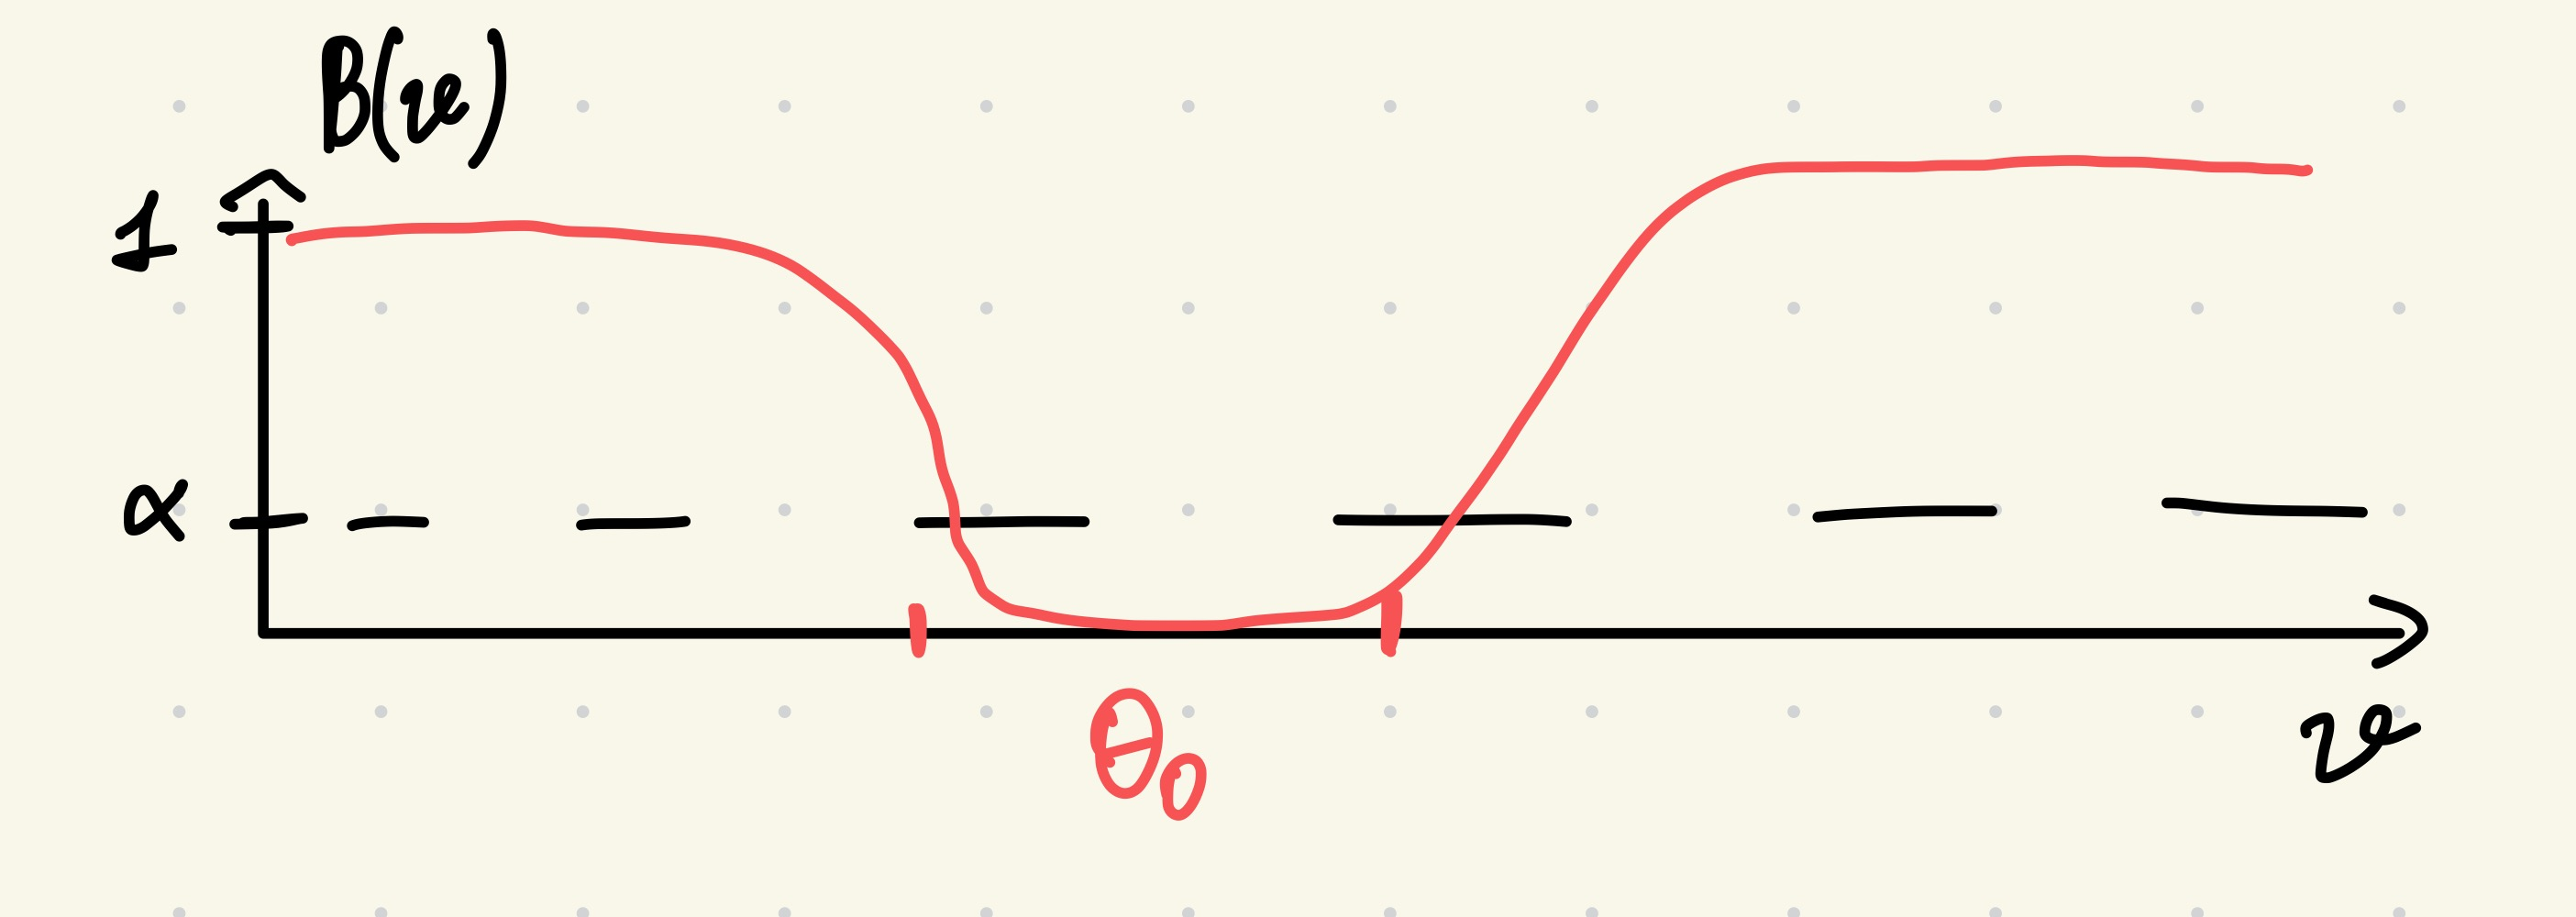
\includegraphics[width=0.5\linewidth]{IMG_1631.jpeg}
        \end{figure}
        \2 Fehler 1. Art -- verwerfen die $H_0$, obwohl sie gilt, soll um egal welche Kosten $\leq \alpha$ bleiben.
        \2 Fehler 2. Art -- verwerfen die $H_0$ nicht, obwohl falsch, Wahrscheinlichkeit $1-\beta(\theta), \theta \in \Theta_1$. Die Wahrscheinlichkeit soll möglichst klein sein.
    \1 Äquivalenz Hypothesentest $\iff$ Konfidenzbereich
        \2 Sei $C(X)$ ein $(1-\alpha)$-Konfidenzbereich für $\theta$. Definiere $\phi(X):= 0$, falls $\theta_0 \in C(X)$ und $\phi(X)=1$, falls $\theta_0 \not\in C(X)$.
    \1 Zusammenfassung:
        \2 Verteilungsfunktion -- p-Werte
        \2 Likelihood --
        \2 Pivot -- Hypothesentest
        \2 Normalapproximation
    \1 Beispiel: Gauß-Modell, $X_1,\ldots,X_n \sim N(m,v)$
        \2 $H_0: m=m_0$
        \2 $(1-\alpha)$-Konfidenzbereich : $C(X)=\{m\in\R : \left|\frac{\overline{X}_n-m}{\sqrt{V_n^* / n}}\right|<q_{1-\alpha}\}$
        definiert einen Hypothesentest zum Niveau $\alpha$, wenn $\phi(X)=1$, falls $|T_n(m_0)|\geq q_{1-\frac{\alpha}{2}}$. Das ist genau der Studentsche $t$-Test.
        \2 $H_0: m=m_0$, $H_1 : m>m_0$
        \2 $C'(X)=\{m\in\R : T_n(m) < q_{1-\alpha}\}$
\end{outline}

\newpage 

\section{Likelihood}

\begin{outline}
\0 Annahmen: entweder $S$ abzählbar, $f_\theta(x)$ Massenfunktion oder $S=\R^d$ und $f_\theta(x)$ Dichtefunktion
    \1 Likelihood-Funktion $L(\theta;x)=f_\theta(x)$ Dichtefunktion von $X$ unter $\theta$; $X$ ist fest.
    \1 log-Likelihood $l(\theta;x)=\log f_\theta(x)$ falls $f_\theta(x)> 0$
\0 Beispiel: Produktmodell $X=(X_1,\ldots,X_n)$, $X$ i.i.d. mit Dichtefunktion $g_\theta$. Dann ist die Likelihood $L(\theta;x)=\prod^n_i g_\theta(x_i)$, log-Likelihood $l(\theta;x)=\sum^n_i \log g_\theta(x_i)$.
\end{outline}

\subsection{Maximum-Likelihood-Prinzip}

\begin{outline}
\0 Konstruiere einen Schätzer $\hat{\theta}=T(X)$ für $\theta$: wähle den Parameterwert $T(x)$, für den der Beobachtungswert $x$ am plausibelsten ist, d.h.
$$L(T(x);x)=\max_{\theta\in\Theta}L(\theta_i;x) \qquad x\in S$$
    \1 Der Schätzer $\hat{\theta}=T(X)$ heißt \emph{Maximum-Likelihood-Schätzer} (MLS) für $\theta$, falls $T(X)\in \operatorname{argmax}_{\theta\in\Theta} L(\theta;x) \forall x\in S$
    \1 \textbf{Beispiel 1}: German tank problem
        \2 $L(N;x)=f_N(x)=\frac{1}{|\Omega_N|}$ für $x\in \Omega_N$ und $0$ sonst. Das ist maximal für $N=\max \{x_1,\ldots,x_n\}$. Unser MLE ist $\hat{N}=\max\{x_1,\ldots,x_n\}$.
\end{outline}

\marginnote[0cm]{6. Vorlesung, 26.04.24}

\begin{outline}
    \1 \textbf{Beispiel 2}: $Bernoulli(p)$, $L(p;X)=P_p(X_1=x_1,\ldots,X_n=x_n)=\prod_{i=1}^n p^{x_i}(1-p)^{1-x_i}$, 
        \2 $l(p,x)=\log(p)\sum_i x_i + \log(1-p)\sum_i(1-x_i)$, optimiere nach $p$ (Ableitung $=0$).\\
    \1 \textbf{Beispiel 3}: Schätzen einer unbekannten WV
        \2 $\Theta$ = alle WVn auf $\hat{a}\in\R^n = \{\overline{p}:\sum p_i = 1\} \in \R^n$ ein Standard-Simplex, $X_1,\ldots,X_n$ unabängig mit Verteilung $p$ unter $P_p$. \2 $L(p;x)=P(X_1=x_1,\ldots,X_n=x_n)=\prod_i p_{x_i} = \prod_{l=1}^k p_l^{h_l}$, wobei $h_l$ = Häufigkeit von $p_l$.
        \2 \textbf{Behauptung:} MLE $\hat{p}$ für $p$ ist $\hat{p}_l= \frac{H_l}{n}$ = relative Häufigkeit von $a_l$ mit Stichprobe $X_1,\ldots,X_n$. \textcolor{orange}{Empirische Verteilung ist MLE für zugrundeliegende WV!} Beweis mit Lagrange.
    \1 \textbf{Beispiel 4}: Gauß-Modell
        \2 $\Theta = \R \times (0,\infty)$, 
        \2 $L(m,v;x)=-\frac{n}{2}\log(2\pi v) - \frac{1}{2v}\sum(x_i-\overline{x})^2 - \frac{n}{2v}(\overline{x}_n-m)^2$
        \2 Schätzen von $m$ bei bekannter Varianz $v$, MLE $\hat{m}=\overline{X}_n$
        \2 Schätzen von $v$ bei bekanntem Mittelwert $m$, MLE empirische Varianz
        \2 Schätzen von $\theta=(m,v)$
            \3 $m=\overline{X}_n$, $v=\frac{1}{n}\sum_i(x_i-\overline{x}_n)^2$
            \3 MLE $\hat{\theta}=(\overline{X}_n,V_n)$ (nicht erwartungstreu in $v$)
\end{outline}

\subsection{Suffiziente Statistiken}

\begin{outline}
\0 Datenreduktion, beinhaltet alle Informationen, die für Rückschlüsse auf $\theta$ relevant sind. Idee: Wahlprognose $X_1,\ldots,X_n \sim Bernoulli(p)$. Für Rückschlüsse auf $p$ reicht es, $\sum X_i$ zu wissen.
    \1 Eine Statistik $T(X)$ heißt \emph{suffizient} für $\theta$, falls $$L(\theta,x)=f_\theta(x)=g_\theta(T(x))h(x) \quad\forall \theta \in \Theta, x\in S$$ 
    mit messbaren Funktionen $g_\theta:\R\ra [0,\infty]$, $h:S\ra[0,\infty]$. Likelihood hängt nur durch $T(X)$ von $\theta$ ab.
    \1 Gilt $h(x)>0$,dann folgt daraus für MLE: $$\operatorname{argmax}_{\theta\in\Theta} L(\theta_i;x)=\operatorname{argmax}_{\theta\in\Theta}g_\theta(T(X)).$$
    und wenn das Maximum eindeutig ist (z. B. falls $l$ strikt konkav), dann ist MLE eine Funktion von $T(x)$.
    \1 \textbf{Lemma}: $T(X)$ ist suffizient, wenn $P_\theta(X=x|T(x)=t)$ nicht von $\theta$ abhängt.
    \1 Als Zweistufenmodell
        \2 Ziehe $T(X)$ aus Verteilung von $T(X)$ (hängt von $\theta$ ab).
        \2 Ziehe $X$ aus Verteilung von $X$ gegeben $T(X)$ (hängt nicht von $\theta$ ab). 
\0 Die Idee: je größer die betrachtete Klasse von Wktsverteilungen, desto mehr Informationen muss die suffziente Statistik enthalten.
    \1 \textbf{Satz}: Rao-Blackwell. Ein beliebiger Schätzer $\hat{g}$ kann verbessert werden, wenn man stattdessen die bedingte Erwartung $\Tilde{g}:=\E{\hat{g}|T(X)}$ betrachtet. 
\end{outline}

\subsection{Exponentielle Familien}

\marginnote[0cm]{7. Vorlesung, 30.04.24}
\begin{outline}
    \1 Definition: $f_\theta(x)=e^{c(\theta) \cdot T(x)+d(\theta)+U(x)}1_A(x)$
        \2 in natürlicher Form, $f_\theta(x)=e^{\theta\cdot T(x)+d(\theta)+U(x)} 1_A(x)$,
        \2 alternative Schreibweise, $f_\theta(x)=\frac{1}{\cZ(\theta)}e^{c(\theta)\cdot T(x)}h(x)$, wobei 
            \3 Normierungskonstante $\cZ(\theta):=e^{-d(\theta)}$, 
            \3 Referenzdichte $h(x)=e^{U(x)}1_A(x)$ 
    \1 Beispiele: Exponentialverteilungen, Bernoulli-, Binomial-, Poisson-Verteilungen, Normalverteilungen.
    \1 In einer exponentiellen Familie ist $T(X)$ eine suffiziente Statistik.
    \1 Wichtige Eigenschaft: Stabilität under Produktbildung.
\marginnote[0cm]{8. Vorlesung, 03.05.24}
    \1 Berechnung von Momenten:
        \2 Momenterzeugende Funktion $M(s):=\E{e^{sT(x)}}=\int e^{sT(x)}f_\theta(x)dx = e^{d(\theta)-d(s+\theta)}<\infty$
        \2 Mit Algebra $M(s)=\frac{\cZ(s+\theta)}{\cZ(\theta)}=e^{d(\theta)-d(s+\theta)}<\infty$
            \3 eine Bedingung an $M(s)$: muss in der Umgebung von $0$ endlich sein
            \3 $\E{T(X)}=\E{\nabla_s e^{sT(X)}|_{s=a}}=\nabla M(0)=-\nabla d(\theta)$
            \3 $\E{T_i(X)T_j(X)}=\ldots$
            \3 $\operatorname{Cov}[T_i(X)T_j(X)]=\ldots$
    \1 \textbf{Satz}: $\hat{\theta}$ ist MLS $\iff$ $\E{T(X)}=T(X)$
    \1 Berechnung des MLS:
        \2 $l(\theta,X)=\log f_\theta (X)=d(\theta)+\theta T(X)+\log h(x)$
        \2 $\nabla l(\theta)=\nabla d(\theta) + T(X)=0 \iff \nabla(\theta)=-T(X) \iff \E{T(X)}=T(X)$. Der MLE ist genau der Parameterwert $\theta$, unter dem $T(X)$ dem Erwartungswert entspricht.
\end{outline}

\subsection{Likelihood-Quotienten-Test}

\begin{outline}
\0 Gegeben ist $H_0: \theta \in \Theta_0$, $H_1: \theta \in \Theta_1$.
    \1 Ein Hypothesentest ist eine Funktion $\phi:S\ra [0,1]$ mit Verwerfenswahrscheinlichkeit $\phi(x)$.
    \1 Der Verwerfungsbereich ist $C(X)=\{x\in S : \phi(x)=1\}$.
    \1 Die Gütefunktion $G(\theta)=\E{\phi(X)}$, Erwartungswert der Wkt, die Nullhypothese zu verwerfen.
    \1 Der Test hat Signifikanzniveau $\alpha$, falls $G(\theta)\leq \alpha \qquad\forall \alpha \in \Theta_0$.
    \1 Die Macht des Hypothesentests ist $G(\theta)$ eingeschränkt auf $\Theta_1$. Kleinere Macht $\implies$ größere Wkt, die Nullhypothese fälschlicherweise nicht zu verwerfen, Fehler 2. Art.
\0 \textbf{Einfacher Likelihood-Quotienten-Test}, feste $\theta_0$ und $\theta_1$:
    \1 Entscheidungsregel: relative Dichte $$R(x)=\frac{L(\theta_1;x)}{L(\theta_0;x)}>c,$$
    \1 Entscheidungsfunktion $\phi = 1_{R(x)>c} + p\cdot 1_{R(x)=c}$
    \1 \textbf{Neyman-Pearson-Lemma}: der LQT ist der mächtigste Test zum Niveau $\alpha$.\\
\marginnote[0cm]{9. Vorlesung, 06.05.24}
\marginnote[0cm]{$\Theta_0$ und $\Theta_1$ sind jetzt ein Bereich, keine feste Parameter}
\0 \textbf{Monotone Likelihood-Quotienten}, $\theta_0\in\Theta_0$ und $\theta_1\in\Theta_1$: 
    \1 nach Definition gilt: 
    $$R(x)=\frac{L(\theta_1;x)}{L(\theta_0;x)}=\frac{\cZ(\theta_0)}{\cZ(\theta_1)} e^{\Large(c(\theta_1)-c(\theta_0)\Large)T(x)},$$
    \1 \textbf{Satz}: für das einseitige Testproblem $H_0 : \theta \leq \theta_0$, $H_1: \theta > \theta_0$ und falls der Likelihood-Quotient streng monoton wachsend in $T(X)$ ist, dann ist LQT $\phi(X)$ der gleichmäßig \emph{mächtigste} Test,
    $$\E{\psi(X)} \leq \E{\phi(X)} $$

\0 \textbf{Allgemeine Likelihood-Quotienten-Tests}, (ad hoc)  
$$R(x)=\frac{\sup \{L(\theta;x) : \theta \in \Theta_1\}}{\sup \{L(\theta;x) : \theta \in \Theta_0\}}$$
\end{outline}

\subsection{Studentsche Konfidenzintervalle und $t$-Test}

\begin{outline}
    \1 Einführung: Gauß-Modell mit unbekanntem Mittelwert und Varianz, Schätzung von $m$.
        \2 Empirischer Mittelwert $\overline{X_n}(\omega)$
        \2 Varianz bekannt: Pivot
        \2 Varianz unbekannt: Studentscher $t$-Test
    \1 $\overline{X}_n\sim N(m,\frac{v}{n})$ und $\frac{n-1}{v}V_n \sim \chi^2(n-1)$
    \1 Verwende Studentsche $t$-Statistik mit $n-1$ Freiheitsgraden, $$T_{n-1}(X)=\frac{\sqrt{n}\cdot (\overline{X}_n - m)}{\sqrt{V_n}}.$$
\marginnote[0cm]{10. Vorlesung, 10.05.24}
    \1 Lemma 2.16: $$f_{\chi^2(n)}\propto x^{\frac{n}{2}-1}e^{-\frac{x}{2}} 1_{(0,\infty)}(x)$$ 
    und 
    $$f_{t(n)}(x) \propto (1+\frac{x^2}{n})^{-\frac{n+1}{2}} (\sim e^{\frac{x^2}{2}} \text{ für } n\ra \infty)¶.$$
\0 Fazit: wir können die Varianz mit der Stichprobenvarianz ersetzen und dabei einen nicht allzu großen Fehler machen. 

\subsection{Anwendung auf Konfidenzintervalle \& Tests}
    \1 ein Test ist \textbf{unverfälscht} zum Niveau $\alpha$, wenn $P(T(X)>c) \leq \alpha$ wenn $H_0$ wahr und $P(T(X)>c) \geq \alpha$ wenn $H_1$ wahr. In anderen Worten, $\E{\phi(\theta_0)}\leq \alpha \leq \E{\phi(\theta_1)}$
    \1 Studentscher $t$-Test ist ein LQT für Gauß-Modell und ist der beste unverfälschte Test i. S. v. oben.
\end{outline}

\newpage

\section{Entropie und Information}

\marginnote[0cm]{11. Vorlesung, 14.05.24}
\begin{outline}
\0 Es geht um die stetige streng konvexe Funktion
$$u(x)=
\begin{cases}
    x\log x & x > 0 \\
    0 & x=0
\end{cases}, \qquad u'(x)=1 + \log x, \qquad u''(x)=\frac{1}{x}$$
\0 Es gilt $u(x)\geq x-1$ und $\min u(x) = \frac{1}{e}\log(\frac{1}{e})=-\frac{1}{e}$.

\begin{figure}
    \centering
    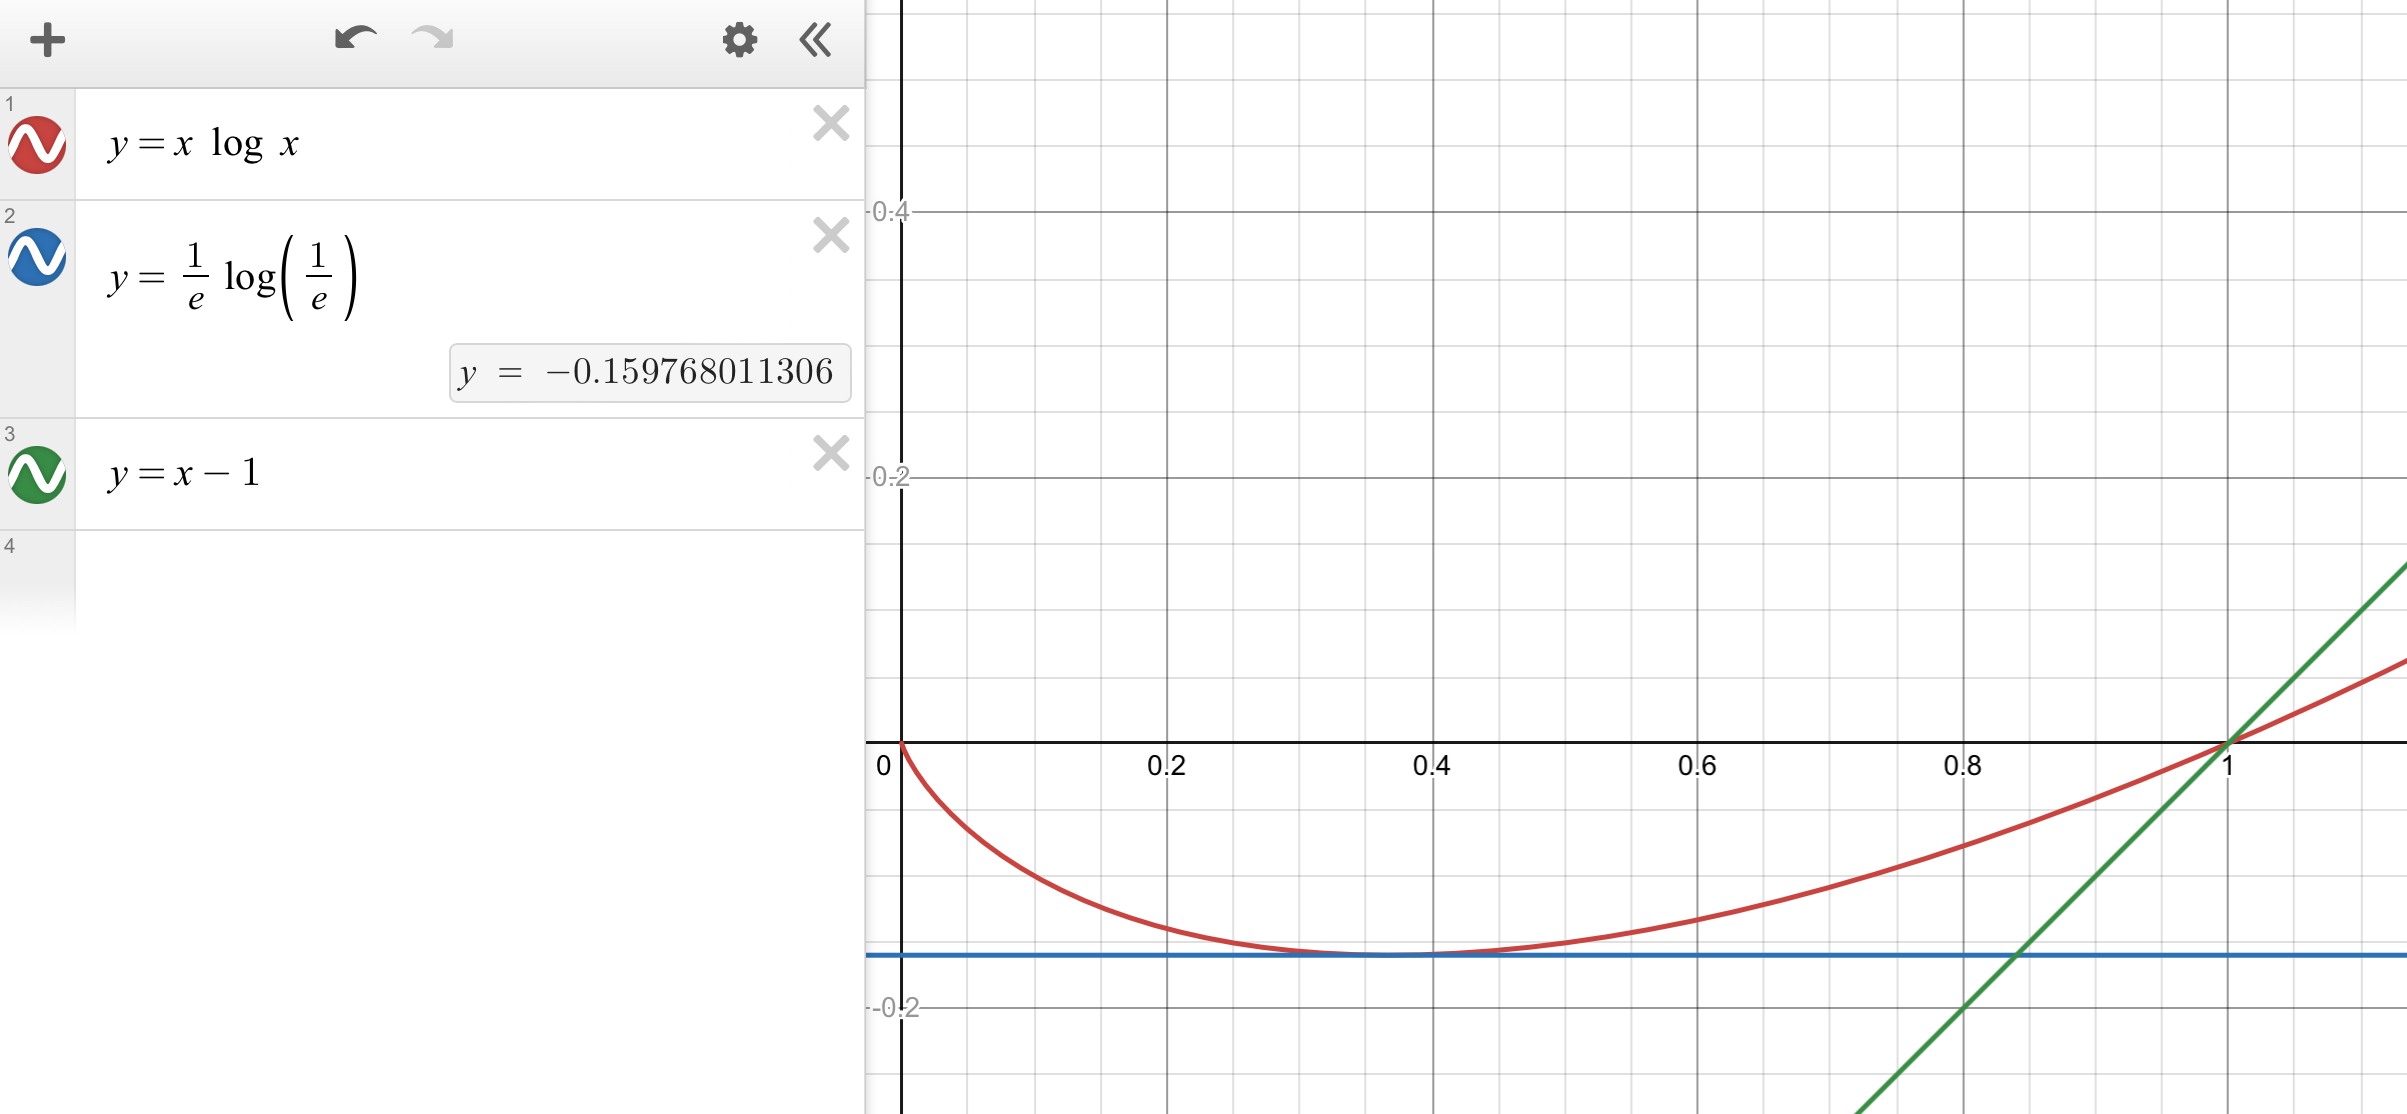
\includegraphics[width=1\linewidth]{IMG_1665.jpeg}
\end{figure}

\subsection{Entropie}

\0 Die \textbf{Entropie} $H(\mu)$ von \textbf{diskreter} Wktsverteilung $\mu$ ist der mittlere Informationsgewinn beim Ziehen einer Stichprobe, also 
$$H(\mu)=-\sum_{x\in S, f(x)\neq 0} f(x)\log f(x)= -\sum_{x\in S, f(x)\neq 0} u(f(x))$$

    \1 Maß für Überraschung oder Informationszuwachs beim Eintritt von Ereignissen der Wkt $p\in[0,1]$ definieren wir als $-\log f(x)$, $f(x)$ ist die Massenfunktion für $\mu$ auf $S$.

    $$H(x)=\underbrace{-\log (f(x))}_{\text{Inform-zuwachs}} \cdot \underbrace{f(x)}_{\text{Wkt. von } x}$$

    \1 Log, weil bei $n$ unabhängigen Stichproben wird aus der Information der Probe $-\log(\prod f_i(x_i))$ ergibt sich der Informationszuwachs als Summe einzelner Beobachtungen $-\sum \log f_i (x_i)$.

    \1 Die Entropie ist immer positiv, da $f(x)\log f(x)$ immer negativ für $f(x)\in [0,1]$. Das gilt nur im abzählbaren Fall!

    \1 Die Entropie ist eine strikt konkave Abbildung auf dem Raum der Wahrscheinlichkeitsverteilungen $WV(S)$.

\0 \textbf{Beispiele}: 

    \1 Bernoulli($p$), Einsetzen ergibt $H(Bernoulli(p))=-p \log p - (1-p)\log (1-p)$, Minimum bei $p=0$ oder $p=1$, Maximum bei $p=0.5$. Sprich, die Verteilung hat minimale Entropie bei $p=\{0,1\}$ und maximale Entropie bei $p=0.5$.

    \1 \textbf{Entropieminima}: Das Dirac-Maß hat minimale Entropie, da $H(\mu) = 0 \iff f(x)\in \{0,1\}$. 

    \1 \textbf{Entropiemaximum}: Die Gleichverteilung hat maximale Entropie wenn $|S|$ endlich ist. Es gilt $H(Unif(S)) = -\log(1/|S|)=\log(|S|)\geq H(\mu)$ für alle anderen $\mu$. Das heißt, Gleichverteilung ist ein ungeordneter Zustand. 

    \1 Entropie kann unendlich sein, falls $S$ wie oben unendlich ist. 

    \1 Entropie der Produktverteilung $H(\mu_1 \otimes \ldots \otimes \mu_n)=\sum_i H(\mu_i)$. Beweis durchs Nachrechnen.

\0 \textbf{Was bedeutet Entropie statistisch?} 
    \1 Nehme $n$ unabhängige Stichproben unter $\mu$. Betrachte relative Häufigkeit $\hat{p}(x_i)=\frac{\# x_i}{n}$ und die empirische Wkt $p(x_1,\ldots,x_n)=\prod_i \hat{p}(x_i)$ als empirische Likelihood-/Dichtefunktion $L(\mu;x_1\ldots x_n)=\prod_i \hat{p}(x_i)$. Gemittelt ergibt sich der mittlere Informationszuwachs als
    
$$\overline{H(X_i)}=-\frac{1}{n} \log(\prod_i \hat{p}(X_i))= - \frac{1}{n} \sum_i \log \hat{p}(X_i).$$
Die Entropie $H(\hat{p})$ ist der mittlere Informationsgewinn bei $n$ Stichproben. Wie verhält sich diese Größe asymptotisch, wenn $n\ra\infty$?

    \1 Satz von Shannon-McMillan I:
    $$-\frac{1}{n}L(\mu;X_1\ldots X_n) \overbrace{\ra}^{n\ra\infty} H(\mu) \text{ almost surely}$$
    Beweis durch GGZ, $\frac{1}{n}l(\mu;X)=\frac{1}{n}\sum_i \log(f(X_i))$, Summanden immer negativ, GGZ anwendbar, also konvergiert die Summe gegen den Erwartungswert $\int \log f d\mu = \sum f(x)\log (f(x)) = -H(\mu)$. \textbf{Entropie ist $\E{H(X)}$}!!!

\0 In der Statistik geht es darum, zwei Wktsverteilungen voneinander zu unterscheiden. Das lässt sich durch relative Entropie quantifizieren. 
\end{outline}

\subsection{Relative Entropie}

\begin{outline}
\0 Gegeben sind zwei Wktsverteiliungen $\mu, \nu$. Die \textbf{relative Entropie} $H(\mu|\nu)$ für absolutstetige Wahrscheinlichkeitsmaße ist nicht symmetrisch und definiert \textbf{bezüglich $\nu$}. 
$$H(\mu|\nu) = \int_{\R^d}\frac{f(x)}{g(x)}\log\left(\frac{f(x)}{g(x)}\right)dx.$$
    \1 $\mu$ muss absolutstetig bzgl. $\nu$ sein,  Notation  $\mu \ll \nu$ 
    \1 dann existiert relative Dichte $\omega=\frac{d\mu}{d\nu}$
        \2 $\mu[B]=\int_B \omega d\nu \quad \forall B \in \cB$ (Lebesgue-Stieltjes?). Kurzschreibweise \enquote{$\mu = \omega d\nu$}. Das ist eindeutig bis auf $\nu$-Nullmengen (man kann eventuell das Maß auf einer Nullmenge ändern, aber ist grds. egal). Die Dichte ist größer gleich Null und strikt größer als Null $\mu$-f.ü, nicht $\nu$-f.ü.
    \2 In dieser Vorlesung sind $S$ abzählbar oder $\R^d$, $\mu,\nu$ mit Massenfunktion/Dichte $f,g$ (sie existieren).
\marginnote[0cm]{$\mu$ hat Verteilung $f$, $ \nu$ hat Verteilung $g$.}
\1 wenn Nullmengen von $\nu$ in Nullmengen von $\mu$ enthalten sind, $\{g=0\}\subseteq \{f=0\}$, dann $\mu \ll \nu$ und es gilt für Dichte 
$$\omega(x)=\frac{d\mu}{d\nu}(x)=
\begin{cases}
    \frac{f(x)}{g(x)} = \frac{L(x,\mu)}{L(x,\nu)} & g(x)>0 \\
    \text{beliebig} & g(x)=0 \text{ (Nullmenge)}
\end{cases}
$$
    \1 Beim Entfernen von $g$ Nullmengen ändert sich $\int f(x)dx$ nach Voraussetzung nicht. Dann kann man $f(x)$ durch $\frac{g(x)}{g(x)}$ ergänzen und $\omega(x)g(x)$ bekommen. Das ist aber genau die relative Dichte $\int \omega d\nu$.

    \1 Rechenregeln:
        \2 $\int h d\mu = \int h \frac{d\mu}{d\nu} \quad \forall h\geq 0$ messbar,
        \2 $m \ll \nu \ll \eta$ impliziert $\mu \ll \eta$ mit $\frac{d\mu}{d\eta} = \frac{d\mu}{d\nu}\cdot \frac{d\nu}{d\eta}$
        \2 Umgekehrt, wenn $m\ll\nu$ und $\frac{d\mu}{d\nu} > 0$ $\nu$-f.ü., dann $\nu \ll \mu$ mit $\frac{d\nu}{d\mu}=\frac{1}{\frac{d\mu}{d\nu}}$.

    \1 \textbf{Relative Entropie} von $\mu$ bzgl. $\nu$ ist definiert als 
    $$H(\mu | \nu):=\int \log\left(\frac{d\mu}{d\nu}\right)d\mu = \int u \frac{d\mu}{d \nu} d\nu \quad \text{wenn } \mu\ll \nu$$
    und ist auch als Kullback-Leibler-Divergenz von $\mu$ bzgl $\nu$ bekannt.

    \1 \textbf{Beispiel:} Sei $\nu$ unser Modell, $\mu$ tatsächliche Verteilung. Dann ist $H(\mu|\nu)= \int \log \frac{f}{g}d\mu = \int (-\log g -(-\log f)) d\mu$ 
        \2 $-\log g$ ist Überraschung in unserem Modell beim Ziehen einer Stichprobe,
        \2 $-\log f$ ist Überraschung beim korrekten Modell,
        \2 die Differenz von beiden ist die Überraschung daraus, dass wir aus dem falschen (Alternativhypothese) Modell eine Stichprobe gezogen haben und das Integral ist ein Mittelwert darüber,
        \2 hätten wir ein korrektes Modell, dann wäre die Überraschung gleich Null.
        
    \1 \textbf{Interpretation 1}: Ist $S$ abzählbar und $\nu$ ein Zählmaß (keine Wktsverteilung), dann gilt $H(\mu|\nu)=\sum f(x)\log(f(x))=-H(\mu)$. Relative Entropie bzgl. des Zählmaßes entspricht also Minus der Entropie. \\

    \1 \textbf{Interpretation 2}: Ist $S$ endlich und $\mu=Unif(S)$, dann gilt $H(\mu|\nu)=\sum f(x) \cdot \log(\frac{f(x)}{1/|S|})=\sum f(x)(\log(f(x))+\log(|S|)=-H(\mu)+\log(|S|)$. Entropie der Wktsverteilung ist gleich der Entropie von der Wktsverteilung verschoben um eine Konstante. Insbesondere gilt $H(\mu |\nu)\geq 0 \implies H(\mu)\leq \log(|S|) = H(Unif(S))$. Also hat Gleichverteilung wirklich eine maximale Entropie. 

\1 Eigenschaften der relativen Entropie:
    \2 $H(\mu |\nu) \geq 0$ und Null gdw $\mu=\nu$
        \3 $H(\mu|\nu)=\int u\frac{d\mu}{d\nu}d\nu$ (interpretiere als $x\log x$) $\geq \int \frac{d\mu}{d\nu}d\nu-\int 1 d \mu = 0$ nach der Ungleichung $u(x)\geq x-1$
        \3 Die Gleichheit in der Abschätzung oben oben gilt gdw $u(\frac{d\mu}{d\nu})=\frac{d\mu}{d\nu}-1$ $\nu$-f.ü. $\iff \frac{d\mu}{d\nu}=1$ $\nu$-f.ü. $\iff \mu=0$.
    \2 $H(\mu_1\otimes\ldots\otimes\mu_n |\nu_1\otimes\ldots\otimes\nu_n)=\sum^n_{i=1}H(\mu_i | \nu_i)$
        \3 ohne Beweis, Übung (LOL)

\0 \textbf{Beispiel}: $H(Bernoulli(a) | Bernoulli(b)) = a \log a/p + (1-a)\log \frac{1-a}{1-p}$
\begin{figure}
    \centering
    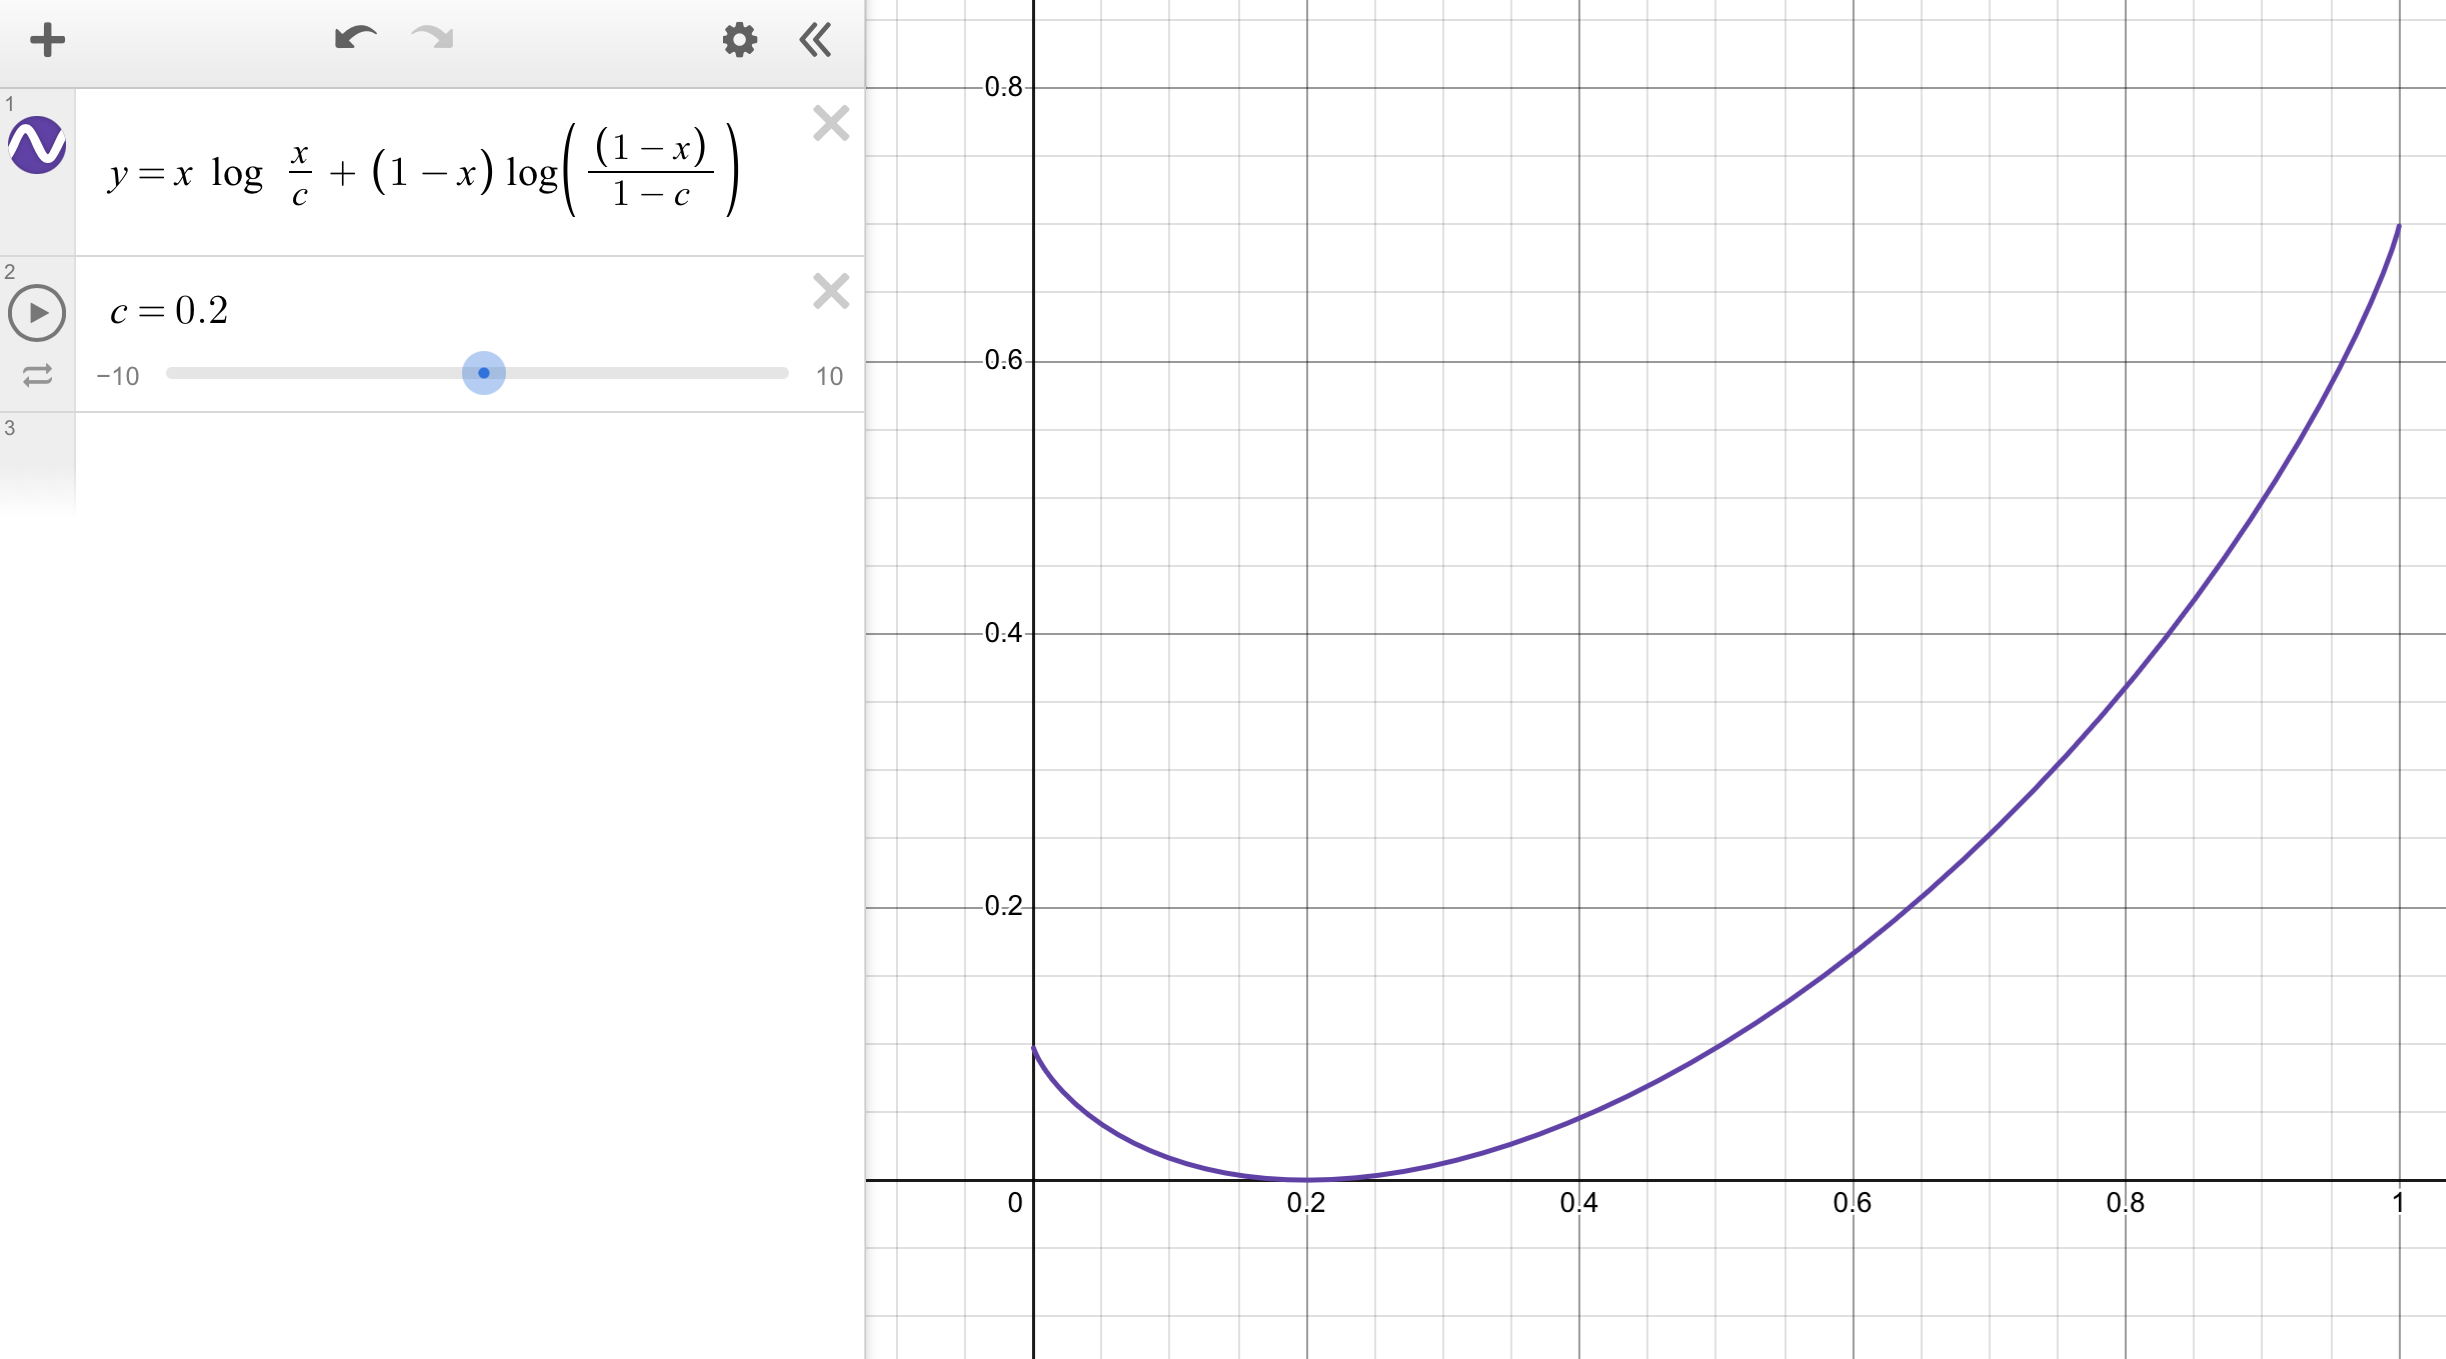
\includegraphics[width=1\linewidth]{IMG_1666.jpeg}
\end{figure}

\0 \textbf{Beispiel}: Normalverteilungen.

\marginnote[0cm]{Prof: \enquote{Was wir hier sehen, ist so eine Art Abstandsbegriff für Wktsverteilungen, der nicht symmetrisch ist.}} 

\subsection{Relative Entropieminimierung unter Nebenbedingung}
\0 \textbf{Anwendung}: Wir wollen für eine Wktsverteilung $\mu_0$ (Referenz) relative Entropie minimieren und eine andere Wktsverteilung finden, gegeben einen festen Abstand $c\in \R$. Mathematisch gilt $H(\mu |\mu_0)=\min \int Td\mu \geq m$. Das ist genau der Fall, wenn die Verteilung aus der exponentiellen Familie ist.\\

\0 \textbf{Exponentielle Familie}: wie bereits vor zwei Wochen gemacht. Wichtig ist der Erwartungswert $m(\theta)=\int T d\mu_\theta$, auch $\mu_\theta \ll \mu_0$ mit $\frac{d\mu_\theta}{d\mu_0}(x)=\frac{Z(0)}{Z(\theta)}e^{\nu T(x)}$
\1 Gibbssches Variationsprinzip: für $\theta\geq 0$ ist $\mu_\theta$ die eindeutige Lösung von dem Minimierungsproblem mit $m=m(\theta)$. 
\marginnote[0cm]{Prof: \enquote{In der Thermodynamik ist die Aussage, dass diese ... Verteilung minimiert die relative Entropie unter den gegebenen Nebenbedingungen.}}
\end{outline}

\marginnote[0cm]{12. Vorlesung, 17.05.24}
\begin{outline}
\0 Recap: relative Dichte wohldefiniert wenn Nenner nicht 0, relative Dichte als Quotient, relative Entropie als Integral, Bezug zu exponentiellen Familien wenn wir Entropie minimieren, global einfach die Verteilung selbst, lokal (mit bestimmten Erwartungswert) immer eine exponentielle Familie. Das möchten wir beweisen.
    \1 Beweis Gibbssches Variationsprinzip. 
        \2 Definiere relative Entropie von $\mu$ bzgl. $\mu_0$, $F(\mu)=H(\mu|\mu_0)-\theta\int T d\mu$.  
        \2 $H(\mu_\theta | \mu_0)=\min \{H(\mu|\mu_0): \mu WV mit \int T d\mu = \int Td\mu_\theta\}$
        \2 $H(\mu|\mu_0)=\int \log\frac{d\mu}{d\mu_0}d\mu=\int \log \frac{d\mu}{d\mu_\theta}d\mu + \int \log \frac{d\mu_\theta}{d\mu_0}d\mu\ldots$
\end{outline}

\subsection{Anwendungen in der Statistik}
\begin{outline}
\0 Wir werden subexponentielle Terme ignorieren. Wenn $a_n, b_n > 0$ zwei Folgen sind, dann sind sie asymptotisch äquivalent, $a_n \simeq b_n$, wenn 
$$\lim_{n\ra\infty}\left(\frac{a_n}{b_n}\right)^\frac{1}{n}=1,$$ 
oder, 
$$\lim_{n\ra\infty}\frac{1}{n}\log\left(\frac{a_n}{b_n}\right)=0.$$ 
    \1 Beispiel: $n^\alpha e^{cn}\simeq n^\beta e^{dn} \iff c=d$.
\marginnote[-1cm]{Prof: wir interessieren uns nur für Abweichungen, die groß genug sind...}
    \1 Setup: $X_1,\ldots,X_n$ i.i.d., mächtigster Test für $X_i\sim \nu$ vs. $X_i\sim \mu$ ist LQT, $$\lambda_n(X_1,\ldots,X_n)=\frac{L_n(\mu,X)}{L_n(\nu,X)}=\prod_i w(X_i)$$ das Produkt der relativen Dichte der zugrundeliegenden Veteilungen. Uns interessiert das asymptotische Verhältnis des LQTs für $n\ra\infty$...

\1 Satz von Shannon-McMillan II:
$$Z_n \simeq e^{nH(\mu|\nu)}, \quad Z_n\simeq e^{-nH(\nu|\mu)}$$
Relative Entropie misst die asymptotische Unterscheidbarkeit von $\mu$ und $\theta$.

\1 Konsistenz: für $n\ra\infty$ die Folge $\hat{\theta}_n := \hat{\theta}(X_1,\ldots,X_n)$ konvergiert zu $\theta$.
\1 Asymptotische Macht von LQT 
    \2 zu einem festen Niveau $\alpha$ gilt, dass $\lim_{n\ra\infty} \frac{1}{n}\log c_n = H(\nu | \mu)$,
    \2 $\lim_{n\ra\infty} \frac{1}{n} \log \mu^n (w_n\leq c_n) \ra -H(\nu | \mu)$
\end{outline}

\subsection{Fisher-Information}
\begin{outline}
    \1 Regularitätsannahmen:
        \2 $\theta \neq \theta' \implies \mu_\theta \neq \mu_{\theta'}$
        \2 $\forall x\in S,\theta\in \Theta$: $f_\theta(x) > 0$
        \2 $f_\theta(x)\in C^3(S)$
        \2 $\int \frac{\partial}{\partial\theta}f_\theta(x)dx =
        \frac{\partial}{\partial\theta} \int f_\theta(x)dx=0$
    \1 Definiere Fisher-Information des parametrischen Modells als 
        $$I(\theta)=\int \frac{1}{f_\theta(x)} |\frac{\partial f_\theta(x)}{\partial\theta}|^2 dx = \int l'(x)^2 f_\theta(x) dx$$
\marginnote[0cm]{13. Vorlesung, 28.05.24}
    \1 Zusammenhang mit relativer Entropie -- infinitesimale Änderung 
    \1 Cramer-Rao-Schranke: für den MSE jedes erwartungstreuen Schätzers gilt
    $$MSE_\nu(\hat{g})=Var_\nu(\hat{g})\geq \frac{g'(\nu)^2}{I(\nu)}.$$
        \2 (Konstante Schätzer haben Varianz 0, die Erwartungstreue ist also notwendig.)
        \2 Beweis: Cauchy-Schwartz für Kovarianz.
\0 \textbf{Beispiele:} Bernoulli, $\hat{p}=X$ mit Varianz $p(1-p)=\frac{1}{I(p)}, g(p)=p$. Optimal! Normalverteilung, $\hat{m}=\overline{X}, Var(\hat{m})=v=\frac{1}{I(m)}$. Optimal! Allgemein: unter welchen Bedingungen haben wir Gleichheit? Wenn die Cauchy-Schwartz-Ungleichung im Beweis scharf ist bzw. Gleichheit gilt. Das ist genau dann der Fall, wenn $l'(\theta, x)$ als affine Funktion von $T(X)$ darstellbar ist, $a(\theta) T(X)+b(\theta)$. 
    \1 Anwendung auf Produktmodell der Normalverteilung, der beste Schätzer im Sinne von oben hat Effizienz $\Omega(1/n)$.
\0 \textbf{Beispiele:} Wieder Normalverteilung, Gleichverteilung auf $(0,\theta)$. Wir haben vor vier Wochen einen supereffizienten Schätzer mit Varianz $O(n^{-2})$ ausgerechnet. Was läuft hier falsch? Die Dichte in diesem Fall ist nicht differenzierbar und die Regularitätsannahme ist damit nicht erfüllt. 
\end{outline}

\marginnote[0cm]{14. Vorlesung, 31.05.24}
\begin{outline}
\0 \textbf{Anwendung von der Informationsungleichung}: Lokationsmodell, $f_\theta(x)=g(x-\theta)$, $g$ ist stetig und symmetrisch. Sei $\hat{\theta}$ ein erwartungstreuer Schätzer für $\nu$, dann nach Informationsungleichung gilt 
$$Var_\theta(\hat{\theta}_n) \geq \frac{1}{nI(\theta)} \forall \theta\in\Theta$$
Es gilt auch $I(\theta)=\E{l'(\theta,X)^2}=\int \frac{g'(x-\theta)^2}{g(x-\theta)}dx=\int\frac{g'(x)^2}{g(x)}dx \forall \theta$
    \1 $I(\theta)$ groß $\iff$ hohe Unterscheidbarkeit $\iff$ kleine Varianz möglich
\0 Definiere \emph{asymptotische Effizienz} als $Var(\hat{\theta}_n)\to \frac{1}{nI(\theta)}, n\mapsto \infty$.
    \1 Stichprobenmittlwert\ldots
        \2 effizient bei der Normalverteilung, nicht asymptotisch effizient bei der Doppelexponentialverteilung, sehr schlecht bei heavy tails
    \1 Stichprobenmedian\ldots
        \2 nicht asymptotisch effizient bei der Normalverteilung, asymptotisch effizient bei der Doppelexponentialverteilung, akzeptabel bei heavy tails. Median ist sehr robust!
\0 Unterschied liegt darin, dass der MLE für NV und DEV genau der Mittlwert/Median ist. \\
\0 \textbf{Asymptotische Normalität von MLE}: Satz von Fisher, Wilks, Wald und Beweis(-skizze).
\end{outline}

\newpage

\section{Empirische Verteilung}
\marginnote[0cm]{15. Vorlesung, 04.06.24}

Nicht-parametrische Modelle. Die empirische Wahrscheinlichkeitsverteilung ist eine Zufallsvariable mit Werten in dem Raum von Wktsverteilungen $WV(S)$, da sie von der Stichprobe abhängt.

\begin{outline}
    \1 empirische Verteilung $L_n$
\0 Die empirische Verteilung $L_n$ ist eine zufällige Wktsverteilung, d. h. $L_n$ ist eine Zufallsvariable mit Werten in $WV(S)$. Für jede disjunkte Zerlegung von $S= B_1\cup B_2 \cup \ldots \cup B_n$ gilt $(H(B_1),H(B_2),\ldots,H(B_n)) \sim Mult(n, \mu(B_1),\ldots, \mu(B_n))$.\\
\0 Wir verwenden $\hat{\mu}_n:=L_n$ als Schätzer für $\mu$ und es gilt $$\E{\hat{\mu}_n(B)}=\mu(B)$$ und $$\Var{\hat{\mu}_n(B)} = \frac{\mu(B)(1-\mu(B))}{n}\leq \frac{1}{4n}.$$
    \1 Satz von Vardarajan: \textbf{Konsistenz} von $L_n$, \url{https://math.stackexchange.com/questions/2602960/proof-of-weak-convergence-of-empirical-measure}
    \1 Dvoretzky–Kiefer–Wolfowitz Ungleichung: \url{https://en.wikipedia.org/wiki/Dvoretzky%E2%80%93Kiefer%E2%80%93Wolfowitz_inequality}
\end{outline}

\subsection{Plug-in Schätzer}

\begin{outline}
    \1 statistisches Funktional $g:P\subseteq WV(S)\ra \R$ 
        \2 Funktion von $L_n$
    \1 Plug-in Schätzer $\hat{g}_n := g(L_n)$ 
        \2 Austausch von der unbekannten Verteilung $\mu$ in der Definition (bzw. im Integral) durch die empirische Verteilung $L_n$ und Übergang zum diskreten Fall (also Summen)
\end{outline}

\subsection{Bootstrap}

\begin{outline}
    \1 Bootstrap-Verfahren
    \1 Bootstrap-Stichprobe
        \2 multinomiales Resampling
    \1 Konfidenzintervall
        \2 Normalapproximation
        \2 empirische Quantile: $[2\hat{g}_n-\hat{q}_{1-\frac{\alpha}{2}}(\hat{g}_n^{(1)}\ldots\hat{g}_n^{(B)}), 2\hat{g}_n-\hat{q}_{\frac{\alpha}{2}}(\hat{g}_n^{(1)}\ldots\hat{g}_n^{(B)})]$
\end{outline}

\marginnote[0cm]{16. Vorlesung, 07.06.24}
Skipped 

\subsection{Anpassungstests}

\marginnote[0cm]{17. Vorlesung, 11.06.24}
Skipped

\marginnote[0cm]{18. Vorlesung, 14.06.24}

\begin{outline}
\1 Normalapproximation der Multinomialverteilung
    \2 degenerierte Normalverteilung $\implies$ Projektion auf Hyperebene
\1 Chiquadrat-Statistik
\1 Satz: Die Approximation konvergiert gegen $N(0,I_{k-1})$ für $n\to\infty$
\1 Satz: Chiquadrat-Statistik konvergiert gegen $\chi^2(k-1)$ für $n\to\infty$
\0 Beweise dazu... sehr lang!

    \1 Anwendung auf Anpassungstests, $H_0 : \mu = \mu_0$
        \2 $\chi^2$-Test: verwerfe, falls $T=n D_2(L_n | \mu_0) \geq c$,
        \2 G-Test: verwerfe, falls $G=nH(L_n | \mu_0) \geq \frac{c}{2}$.
        \2 Beide Tests erfüllen asymptotisch die Niveaubedingung für $n\to\infty$ falls $c=q_{1-\alpha, \chi^2(k-1)}$
\marginnote[0cm]{$2G$ ist wie $T$}
\0 Ergänzung: hier testen wir, ob die Wahrscheinlichkeitsverteilung die eine Wktverteilung ist. Eigentlich möchten wir testen, ob es eine Verteilung aus gegebener endlichdimensionalen Familie ist $\implies$ der Anpassungstest für parametrische Familien, wobei $H_0 : \mu \in \{\mu_\nu : \theta \in \Theta\}$ eine $d$-dimensionale Mannigfaltigkeit. G-Test mit Parameterschätzung. Satz von Wilks: unter der Annahme konvergiert $P\circ (2G)^{-1}$ gegen $\chi^2(k-1-d)$.
\marginnote[0cm]{Wichtig: wir haben nur endlich viele Zustände.}
    \1 Alternative zu Anpassungstests: Konfidenzbereich für $\mu$.
        \2 für Multinomialverteilung bestimme also $k$ Konfidenzbereiche für Binomialverteilung\ldots
        \2 Vorteil: Kontrolle über jeden einzelnen Parameter
        \2 Nachteil: für $n=10$ müssen einzelne Konfidenzbereiche zu $\frac{\alpha}{10}$ bestimmt und geschnitten werden. Brauche mehr Stichprobenwerte, um dasselbe Niveau zu erreichen. (\enquote{Bonferroni-Korrektur}).
\end{outline}

\marginnote[0cm]{19. Vorlesung, 18.05.24}

\begin{outline}
    \1 Satz von Glivenko-Cantelli
    \1 Wie testet man auf Normalverteilung? Weitere Anpassungstests:
        \2 Kolmogorov-Smirnov-Test
        \2 Lilliefors-Test auf Normalverteilung
            \3 $\beta$ ist skaleninvariant
            \3 Probleme mit tails
        \2 Anderson-Darling-Test
        \2 Abweichungen in tails sind nur schwer erkennbar. Alternative: wir verwerfen, falls ein Integral größer $\varepsilon$ ist.
\0 Anmerkung: kein Anpassungstest ist perfekt. Mehrere Tests ausprobieren.
\end{outline}

\subsection{Robuste Verfahren}

\begin{outline}
\0 $\mu$ auf $\R$, $X_1,...,X_n \sim \mu$ i.i.d.
    \1 ein fehlender Datenwert kann $\overline{X}_n$ beliebig verfälschen = nicht robust
    \1 besser ist z. B. der Median $q_\frac{1}{2}$, Ordnungsstatistik = robust
\0 Wir charakterisieren Robustheit von $T_n$ bei $(x_1,\ldots,x_n)$ über:
    \1 Bruchpunkt \[\varepsilon_n(X)=\frac{1}{n}\max_{k\in\{0,1,\ldots,n\}}\{\sup_{y_i\neq x_i k-mal} | T_n(y_1,\ldots,y_n)|<\infty\}\]
    \1 asymptotischen Bruchpunkt $\varepsilon := \liminf_{n\to\infty} \varepsilon_n(X)$
    \1 die Sensitivitätsfunktion
    \1 die Einflussfunktion
\0 Robuste Konfidenzintervalle für Quantile
    \1 Schätze $q_\gamma$ mit Plugin-Schätzer $\hat{q}_\gamma = X_{(n\gamma)}$. Bestimme Konfidenzintervall 
    \1 Satz: die Wkt, dass das Gamma-Quantil zwischen zwei Ordnungsstatistiken liegt, beträgt die Differenz der Verteilungswerte. 
        \2 Verteilungsunabhängige Konfidenzintervalle! Großer Vorteil.
\0 Robuste Konfidenzintervalle für Tests
    \1 Test für Median von zwei Stichproben
        \2 Option 1, Mittelwert: $t$-Test. Probleme: keine Normalverteilung, Ausreißer/Messfehler,
        \2 Option 2, Median: verwerfe $H_0$ falls $X_{(k)}>0$. Pearsons Vorzeichentest. Vorteil: sehr robust, unabhängig von der Verteilung. Nachteil: Größe der $X$ spielt keine Rolle.
        \2 Option 3, Wilcoxon-Signed-Rank-Test:
\end{outline}

\marginnote[0cm]{20. Vorlesung, 21.06.24}

\section{Zusammenhang mehrerer Merkmale}

\subsection{Binäre Merkmale: Chancenquotienten und Vierfeldertafeln}

\marginnote[0cm]{21. Vorlesung, 25.06.24}

\begin{outline}
    \1 $Chance(A):=\frac{P(A)}{P(A^C)}=\frac{P(A)}{1-P(A)}$
        \2 nichtlineare Transformation $p \mapsto \frac{p}{(1-p)}$
    \1 Chancenquotient $\rho:=\frac{p_{11}p_{00}}{p_{10}p_{01}}=\frac{Chance(X=1 |Y=1)}{Chance(X=1 |Y=0)},$
        \2 Aus $\rho =1$ folgt $X,Y$ unabhängig und $p_{kl}=p_{k+}p_{+l}$
    \1 Schätzer für $\rho$: Plug-in Schätzer $\hat{\rho}$
    \1 Konfidenzintervall für $\rho$
        \2 Modell: $(H_{11}, H_{10}, H_{01}, H_{00}) \sim Mult(N,p_{11},p_{10},p_{01},p_{00})$ 
\marginnote[0cm]{22. Vorlesung, 28.06.24}
\marginnote[0cm]{Dümbgen, 7.5}
    \2 Dieselben KI wie beim \textbf{Fischers exakten Test} mit Konfidenzintervallen. Idee: gegeben $\rho$, können wir die bedingte Wkt. $p(H_{11} |H_{1+})$ und $p(H_{11} |H_{+1})$ ausrechnen.\\
    \begin{tabular}{|l|c|c|c|}
    \hline
    \multicolumn{1}{|c|}{\multirow{2}{*}{Haarfarbe}} & \multicolumn{3}{c|}{Augenfarbe} \\
    \cline{2-4}
     & grün & nicht grün & \multicolumn{1}{c|}{} \\
    \hline
    rot & 14 & 57 & 71 \\
    \hline
    nicht rot & 50 & 471 $H_{00}$ & 521 \\
    \hline
     & 64 & 528 & 592 N \\
    \hline
    \end{tabular}
    \2 Lemma: $p(H_{11} |H_{+1}=l, H_{1+}=n) = C_{n,l,N,\rho}\binom{n}{x}\binom{N-n}{l-x}\rho^x$ und die Konstante $C$ hängt nicht von $x$ ab.
    \2 Wir können aus diesen Wkten die Konfidenzintervalle für $\rho$ herleiten. Bedingte Wkt => Verteilungsfunktion => Konfidenzschranken über Umkehrfunktion
    \2 Bei diesem Test typisch ist $H_0 : \rho = 1$, $H_1 : \rho > 1$.
\1 \textbf{Vierfeldertafeln, modifiziertes Modell}.
    \2 Im Unterschied zur oben sind $n_1, n_2$ fest vorgegeben.\\
    \begin{tabular}{|l|c|c|c|}
    \hline
    & Besserung & keine Besserung & \\
    \hline
    Medikament & $H_{11}$ & $H_{12}$ & $n_1$ \\
    \hline
    Placebo & $H_{21}$ & $H_{22}$ & $n_2$ \\
    \hline
    & $H_{+1}$ & $H_{+2}$ & $N$ \\
    \hline
    \end{tabular}
    \2 Modell: $H_{11}\sim Bin(n_1,p_1), H_{21}\sim Bin(n_2,p_2)$ unabhängig.
    \2 Wie oben.
\end{outline}

\subsection{Test auf Unabhängigkeit/Assoziation}
\begin{outline}
\0 Gegeben $X_{1\leq k \leq n}$ und $Y_{1\leq l \leq N}$ entscheide, ob die gemeinsame Verteilung das Produkt der Randverteilungen ist, d. h. wenn $p_{kl}=p_k p_l=:\hat{p}_{kl}$ für alle $k,l$.
    \1 Die Nullhypothese $H_0 : p=\hat{p}$
    \1 Methode 1, multiple Tests: Fishers exakter Test für jeden $k$ und $l$
    \1 Methode 2, Chiquadrat-Test auf Unabhängigkeit: schätze $\chi^2$-Divergenz $$\chi^2(p|\overline{p})=\sum_{k,l}\left(\frac{p_{kl}}{\overline{p_{kl}}}-1\right)^2 p_{kl}=\sum_{k,l}\frac{p_{kl}^2}{\overline{p_{kl}}}-1$$
    Die Schätzung machen wir mit dem Plug-In Schätzer (empirische Verteilung). Unter Nullhypothese ist der Wert Null.
        \2 Berechnung des p-Werts: entweder exakt (bei kleinen Datensätzen) oder Bootstrap. 
        \2 Alternativ kann man Divergenz durch relative Entropie ersetzen.
    \1 $\chi^2$-Approximation ($N$ groß) mit $(k-1)(l-1)$ Graden.
        \2 Nachrechnen bestimmter Eigenschaften der $\chi^2$-Verteilung
\end{outline}

\subsection{Permutationstests}

\marginnote[0cm]{23. Vorlesung, 02.07.24}
\marginnote[0cm]{Dümbgen 8.1-8.3}

\begin{outline}
    \1 $(H'_0):$ \textbf{bedingte Austauschbarkeit} von $Y$ gegeben $X$, wenn für $\pi\in Sym(n)$ gilt $(X,\pi Y)\sim (X,Y)$.
    \1 Lemma: Sei $\pi$ zufällige Permutation, dann gilt für alle feste $x,y$, dass Erwartungswert der Häufigkeiten unter $\pi$ dem naiven Produktmaß entspricht. Der Erwartungswert der Statistik beträgt $\frac{N}{N-1}(k-1)(l-1)$.
    \1 Satz: $\ldots$
\0 \textbf{Ziel:} Untersuchen, ob die ZV unter Permutation invariant in der Verteilung sind. Gegeben ist eine Permutation $\pi\in G$, dabei $G$ eine Untergruppe von $Sym(n) \implies$ $G$-Invarianztest.
    \1 Test auf identische Verteilung von $X,Y$
        \2 $\pi(X,Y) = (\pi X, \pi Y)\sim (X,Y)$
    \1 Test auf Unabhängigkeit $X,Y$
        \2 bedingte Austauschbarkeit $\pi(X,Y)=(X,\pi Y)$
    \1 Test auf Vorzeichensymmetrie 
        \2 Tendenz für positive/negative Vorzeichen
\0 Konstruktion von Tests via $G$-Symmetrie. Sei $T$ eine beliebige Statistik, $(x,y)\in S^{n+m}$ Datenvektor. Definiere 
    \1 linksseitiger $p$-Wert: $p_l^G(x,y) = \frac{|\{\pi \in G: T(\pi(x,y))\leq T(x,y)\}|}{|G|}=P(T(\pi(x,y)) \leq T(x,y))=F_{\{T(\pi(x,y))\}} (T(x,y))$.
    \1 Berechnung von $p_l^G(x,y)$. Abzählen (wenn $G$ klein), Monte-Carlo.
    \1 Satz: unter $(X,Y)\sim \pi(X,y)$ gilt $p_l^G(X,Y)\leq \alpha$ kann höchstens mit Wkt. $\alpha$ gelten.
\0 Beispiel 1: Test auf identische Verteilung, $G=Sym(n+m), T(X_1,...,X_n,Y_1,...,Y_m)=|M_X-M_Y|$, dabei sind $M_X,M_Y$ Mittelwerte/Mediane/... von $X$ und $Y$.\\
\0 Beispiel 2: Test auf Unabhängigkeit, $G=Sym(n), (X_n,Y_n)$ aus $\{0,1\}\times \R $ und $\pi(X,Y)=(X,\pi Y), T(X,Y)=\sum_i 1_{X_i=1} R_i$. Dann könnte man erkennen, ob eventuell kleine/große Ranks von $Y$ überwiegen.
\end{outline}

\section{Regression}

\subsection{Einfache lineare Regression}
\marginnote[0cm]{24. Vorlesung, 05.07.24}

\subsection{Lineare Modelle}
\marginnote[0cm]{25. Vorlesung, 09.07.24}

\begin{outline}
    \1 Modell: $Y=\sum^d_k \omega_k X^{(k)}+ \varepsilon = A\omega + \varepsilon$
        \2 Beobachtung $Y:\Omega \ra \R^n$
        \2 unbekannte Parameter $\omega_1,\ldots,\omega_d \in \R$
        \2 Störgrößen $\varepsilon : \Omega\ra\R^n$
        \2 Design-Matrix $A=(X^{(1)}, \ldots, X^{(d)})$ eine $n\times d$-Matrix mit Rang $d$
    \1 Beispiele: einfache Regression, multiple lineare Regression, polynomielle Regression, Einstichproben-Lokationsmodell, $\ldots$
    \1 Beispiel Mehrstichprobenmodell: Vergleich von $p$ verschiedenen Populationen, z. B. Ertrag bei $p$ verschiedenen Düngersorten.
        \marginnote[0cm]{$(i=1, \ldots, p; k=1,\ldots,n_i)$,\\ $n_i$ Anzahl Stichproben in Gruppe $i$}
        \2 Response $Y_{ik}=m_i + \varepsilon_{ik}$ von Objekt $k$ in Gruppe $i$
        \2 $A=\begin{pmatrix}
            1_{n_1} & 0 & 0\\
            0 & \ddots & 0\\
            0 & 0 & 1_{n_p}
        \end{pmatrix}$, $1_{n_i}=\begin{pmatrix}
            1 \\
            \vdots \\
            1
        \end{pmatrix} \in \R^{n_i}$
        \2 Idee: ANOVA, vergleiche die Varianz zwischen den Gruppen mit der Varianz innerhalb der Gruppen, $H_0 : m_1 = \ldots = m_p$. 
        \2 Vergleiche $\hat{V}_{ZG}$ und $\hat{V}_{iG}$
        \2 Gauß-Fall: $\frac{\hat{V}_{ZG}}{\hat{V}_{iG}} \sim \frac{\frac{v}{p-1}\sum^{p-1}_{i=1} Z_i^2}{\frac{v}{n-p}\sum^{n-1}_{i=p}Z_i^2} = F_{p-1,n-p}$ und $Z_i\sim N(0,1)$ unabhängig.
        \2 Die Verteilung von $F_{p-1,n-p}$ heißt Fisher-Verteilung mit $p-1$ und $n-p$ Freiheitsgraden.
\0 \textbf{Schätzer für $\omega$}: $Y=A\omega + \varepsilon$ 
    \1 kann nicht perfekt klappen, $\dim A < \dim Y, d<n$
    \1 $L:=Range(A)= \{A\omega : \omega \in \R^d\}$
    \1 $\pi:\R^n \ra L$ orthogonale Projektion auf $Range(A)$
    \1 Lemma: $A^\top A\in \R{d\times d}$ ist invertierbar und $\Pi = A(A^\top A)^{-1}A^{\top}$
    \1 Ansatz 1: Kleinste Quadrate
        \2 Minimiere $||Y-A\omega||^2=||Y||^2 - 2 (A^\top y)\cdot \omega + \omega \cdot A^\top A \omega != \min$
        \2 Berechne den Gradienten $\nabla = -2A^\top y + 2 A^\top A \omega != 0$
        \2 $A^\top A \omega = A^\top Y$ Normalengleichungen und $\hat{\omega} = (A^\top A)^{-1}A^\top Y$ Minimum, denn Hesse-Matrix $=2A^\top A$ ist symmetrisch positiv definit.
        \2 Bemerkung: $A\hat{\omega}=\Pi Y$ nach Lemma
\end{outline}
\subsection{Andrere Regressionsverfahren}

\section{Bayes-Statistik}

\subsection{Ansatz der Bayesschen Statistik}

\subsection{Gibbs-Sampling}

\section{Klausurvorbereitung}
\begin{outline}
\0 Liste A1)
    \1 Verteilungsfunktion
    \1 Konfidenzintervall
    \1 Median  
        \2 \url{https://math.stackexchange.com/questions/113270/the-median-minimizes-the-sum-of-absolute-deviations-the-ell-1-norm}
    \1 Chiquadrat-Verteilung
    \1 Empirische Verteilung
    \1 Normalverteilung
        \2 \url{https://en.wikipedia.org/wiki/68%E2%80%9395%E2%80%9399.7_rule}
    \1 Binomialverteilung
    \1 Studentsche $t$-Statistik
    \1 Exponentialverteilung
        \2 \url{https://stats.stackexchange.com/questions/2092/relationship-between-poisson-and-exponential-distribution}
\end{outline}
\end{document}